% Chapter 6

\chapter{Compton Photon Target}
\captionsetup{justification=justified,singlelinecheck=false}

\label{Ch:Compton_Laser}

\lhead{Chapter 6. \emph{Compton Photon Target}} 
The Compton polarimeter, built in Hall C for the \Qs experiment, measured the polarization of the electron beam by probing it with a circularly-polarized green laser and measuring the difference of e$\gamma$ scattering rates between the two helicity states of the electron beam. Figure \ref{fig:compton_layout} shows the basic components of the polarimeter and its operation is explained in Section \ref{sctn:compton}. The photon target, produced and controlled on the laser table and injected into the electron beam pipe at the interaction region, is a critical subsystem common to both photon and electron detector polarimetry measurements. The production, control and measurement of the properties of the photon target, one of the key contributions of the author to the \Qs experiment, is the subject of this chapter. Although Compton polarimetry data exists for part of Run 1, issues in the analysis for both photon and electron detectors produce larger uncertainties, and at the time of this writing, it appears that the electron beam polarization for Run 1 will be determined by the M\o ller polarimeter. A number of hardware, software and operational changes made before Run 2 make this a much higher quality dataset and although occasional mention of methods and issues during Run 1 will be made, all analyses and calculations shown in this chapter will be for the Run 2 data set.

The Compton scattering asymmetry between the two electron helicity states is calculated as 
\begin{equation}
A_{meas}=\frac{Y_R-Y_L}{Y_R+Y_L},
\label{eq:ameas}
\end{equation}
where $Y_{R(L)}$ are the background subtracted scattering rates for right and left electron spin states. This measured asymmetry is a product of three components given by
\begin{equation}
A_{meas}=P_{\gamma}P_eA_{Compton},
\label{eq:asymtopol}
\end{equation}
where $P_{\gamma (e)}$ are the photon (electron) polarizations and $A_{Compton}$ is the analyzing power precisely determined from the expected asymmetry from quantum electrodynamics convoluted with a carefully measured detector response. The electron beam polarization is calculated from this equation with all other terms measured.

Since the yields (integrated rates) in Equation \ref{eq:ameas} are background subtracted, backgrounds in the Compton detectors are a source of potentially large systematic errors. The larger the signal to background ratio, the smaller the contribution of this error. Equation \ref{eq:asymtopol} clearly illustrates the importance of a highly polarized light source and an accurate determination of its polarization. The remainder of this chapter is devoted to these two issues: the creation of a high power target for increasing signal to background\footnote{Higher target power also allows faster measurements of statistically accurate polarizations necessary for real time polarization tracking.} and the setup and accurate determination of its polarization.

\section{The Fabry-Perot Optical Cavity}
The photon target for the Compton polarimeter was produced using a Coherent Verdi-V10 (\cite{Verdi10}) laser delivering $>$10~W of green light (532~nm) mode-matched to an 84.2~cm long Fabry-Perot optical cavity. Mode-matching an optical cavity refers to the process of shaping and aligning the laser to match the allowed transverse resonating modes of the optical cavity. The Coherent Verdi-V10 produced a high quality Gaussian beam with $M^2<1.1$. Although the propagation of Gaussian beams is beyond the scope of this thesis, a few specifics will be provided to facilitate the discussion of optical mode-matching.

Gaussian beams have a transverse intensity profile that is approximately normal, meaning that most of their power propagates in the TEM$_{00}$ mode. Perfect Gaussian beams can be characterized completely by two parameters: $w(z)$, the $2\sigma$ width of the transverse intensity distribution, and $R(z)$, the radius of curvature of the laser-beam wavefront where $z$ is the distance along the beam propagation path. The two parameters expressed in terms of the laser wavelength $\lambda$ and waist $w_0$ (the minimum laser width $w$) are given as
\begin{equation}
R(z)=z\left[1+\left(\frac{\pi w_0^2}{\lambda z}\right)^2\right]
\label{eq:R}
\end{equation}
and
\begin{equation}
w(z)=w_0\sqrt{1+\left(\frac{\lambda z}{\pi w_0^2}\right)^2}.
\label{eq:w}
\end{equation}
From these equations it is obvious that $z$ is measured relative to where the beam wavefront is flat $R(0)=\infty$ and that at this position the beam is also at its minimum width $w_0$. From Equation \ref{eq:w} one can see that $w(z)$ asymptotically approaches a linear divergence in $z$ with an angle $\theta=\lambda/\pi w_0$ with respect to $z$ (small angle approximation).

Realistic, non-ideal, Gaussian beams require a third parameter, $M^2>1$, which measures the deviation of a laser from the ideal Gaussian TEM$_{00}$ propagation mode. $M^2=1$ describes an ideal Gaussian beam. The presence of a non-unity $M^2$ modifies the equations \ref{eq:R} and \ref{eq:w} giving 
\begin{equation}
w_M(z)=w_{0M}\sqrt{1+\left(\frac{\lambda z M^2}{\pi w_{0M}^2}\right)^2}
\label{eq:w_m}
\end{equation}
and
\begin{equation}
R_{M}(z)=z\left[1+\left(\frac{\pi w_{0M}^2}{\lambda z M^2}\right)^2\right],
\label{eq:R_m}
\end{equation}
where $w_{0M}$ is the measured minimum waist. The Coherent Verdi-V10 laser output was a 10~W highly Gaussian beam with quoted $M^2<1.1$, although measurements of the laser $M^2$ on the table often gave higher values in the 1.2 - 1.3 range. This decrease in laser-beam quality is not surprising given the observation of thermal lensing in optical elements on the laser table.

One final thing to note is, that for a beam that is not circular, two independent sets of equations are required: a $w_M(z)$ and an $R_M(z)$ for two orthogonal transverse dimensions ($x$ and $y$ for example). This means that the horizontal profile of the beam will propagate independently of the vertical profile and they may not even come to a waist at the same $z$ location. 

Gaussian beams are shaped using lenses, and linear transformation rules similar to those of geometric optics can be formulated to model the beam transport (see reference for details \cite{Kogelnik}). Mode-matching to an optical cavity is the process of shaping and aligning a laser such that its electric field distribution matches a particular resonating mode of the optical cavity. Although a laser is typically matched to the fundamental Gaussian mode of the optical cavity, misalignments and poor mode-matching solutions will allow other modes to propagate. Cavity resonating modes can be expanded in either cylindrical or Cartesian bases; however, the simplest basis depends upon the type of mode mismatch as explained below\cite{Anderson}. \\
1. Transverse Cartesian Basis:\\
This basis is made up of a Gaussian multiplied by Hermite polynomials and produces an intensity pattern given by 
\[I_{mn}(x,y)=I_0\left[H_m\left(\frac{\sqrt{2}x}{w}\right)e^{-x^2/w^2}\right]^2\left[H_n\left(\frac{\sqrt{2}n}{w}\right)e^{-y^2/w^2}\right]^2,
\] 
where $w$ is the mode transverse spot size and $H_{m(n)}$ are the Hermite polynomials for the $x~(y)$ dimensions. The indices $m$ and $n$ indicate the number of nulls in the intensity distribution in the $x$ and $y$ directions respectively. This basis is useful for describing resonator modes that exhibit broken cyclindrical symmetry. Examples of this type of broken symmetry are mirror angle misalignment, laser position or angle offsets from the cavity axis and the presence of linear polarization. The lowest order Hermite-Gaussian cavity modes can be seen in Figure \ref{fig:hermite_modes}.

\begin{figure}
\begin{center}
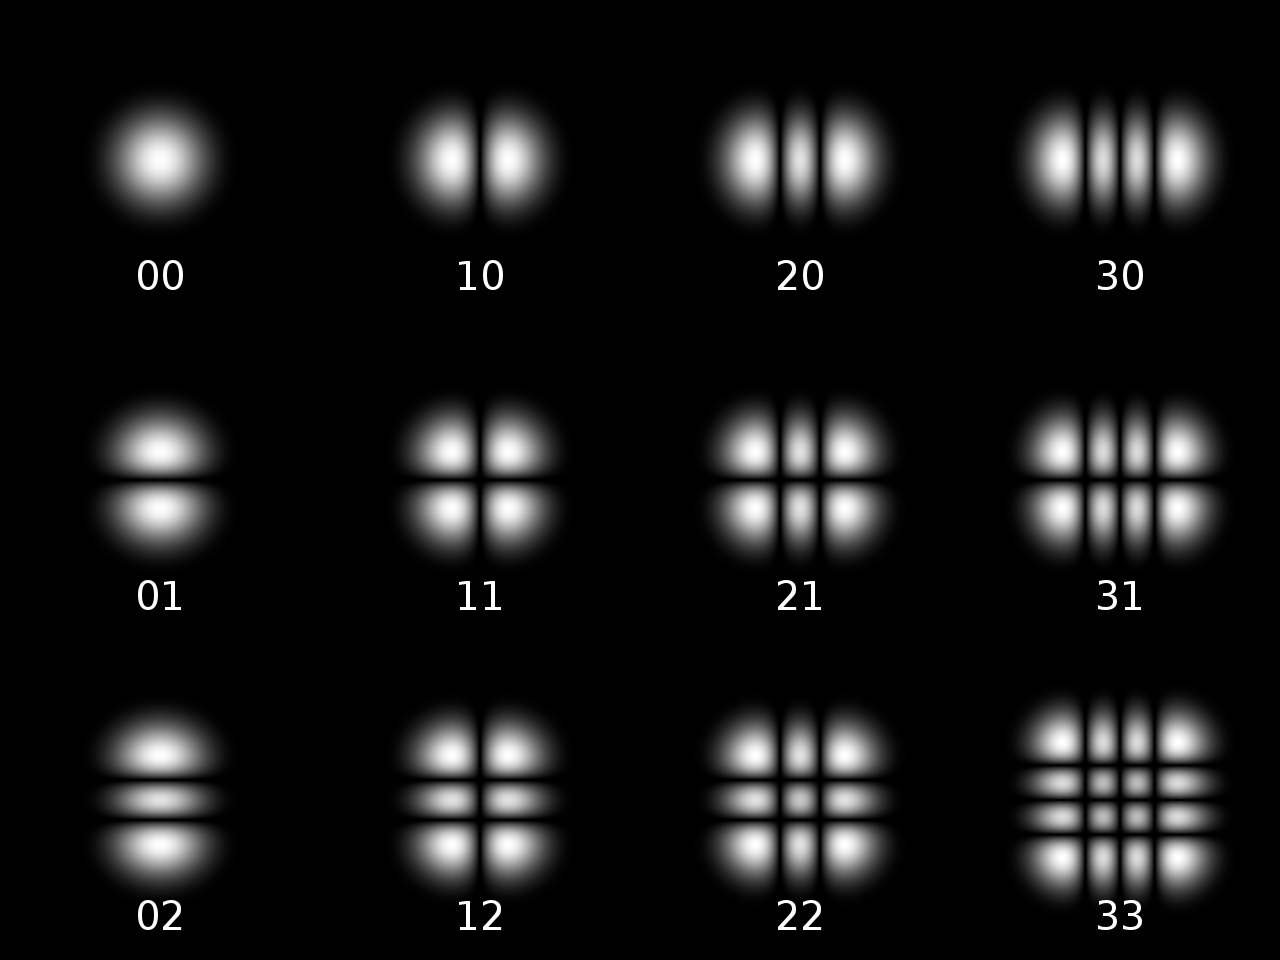
\includegraphics[width=3.2in]{./Pictures/Hermite-gaussian.png}
\caption{\label{fig:hermite_modes}Hermite-Gaussian resonator modes for an optical cavity. Figure courtesy of {\it Wikimedia Commons}.}
\end{center}
\end{figure}

2. Transverse Cylindrical Basis:\\
This basis is composed of a Gaussian multiplied by Laguerre polynomials and produces a transverse intensity distribution given by
\[
I_{\rho l}(\rho ,\phi )=I_0\rho^l\left(L_p^l(\rho)\right)^2\cos^2(l\phi)e^{-\rho},
\]
where $\rho$ and $\phi$ are polar coordinates, $L_p^l$ is the order-$p$ Laguerre polynomial with index $l$, and $w$ is the transverse spot size of the resonator mode. This basis is useful for describing mismatches that preserve cylindrical symmetry such as a mismatch of the radius of curvature of the laser to the cavity mirrors or a laser waist that is not centered on the cavity resonator mode waist. The lowest order Laguerre-Gaussian cavity modes can be seen in Figure \ref{fig:laguerre_modes}.

\begin{figure}
\begin{center}
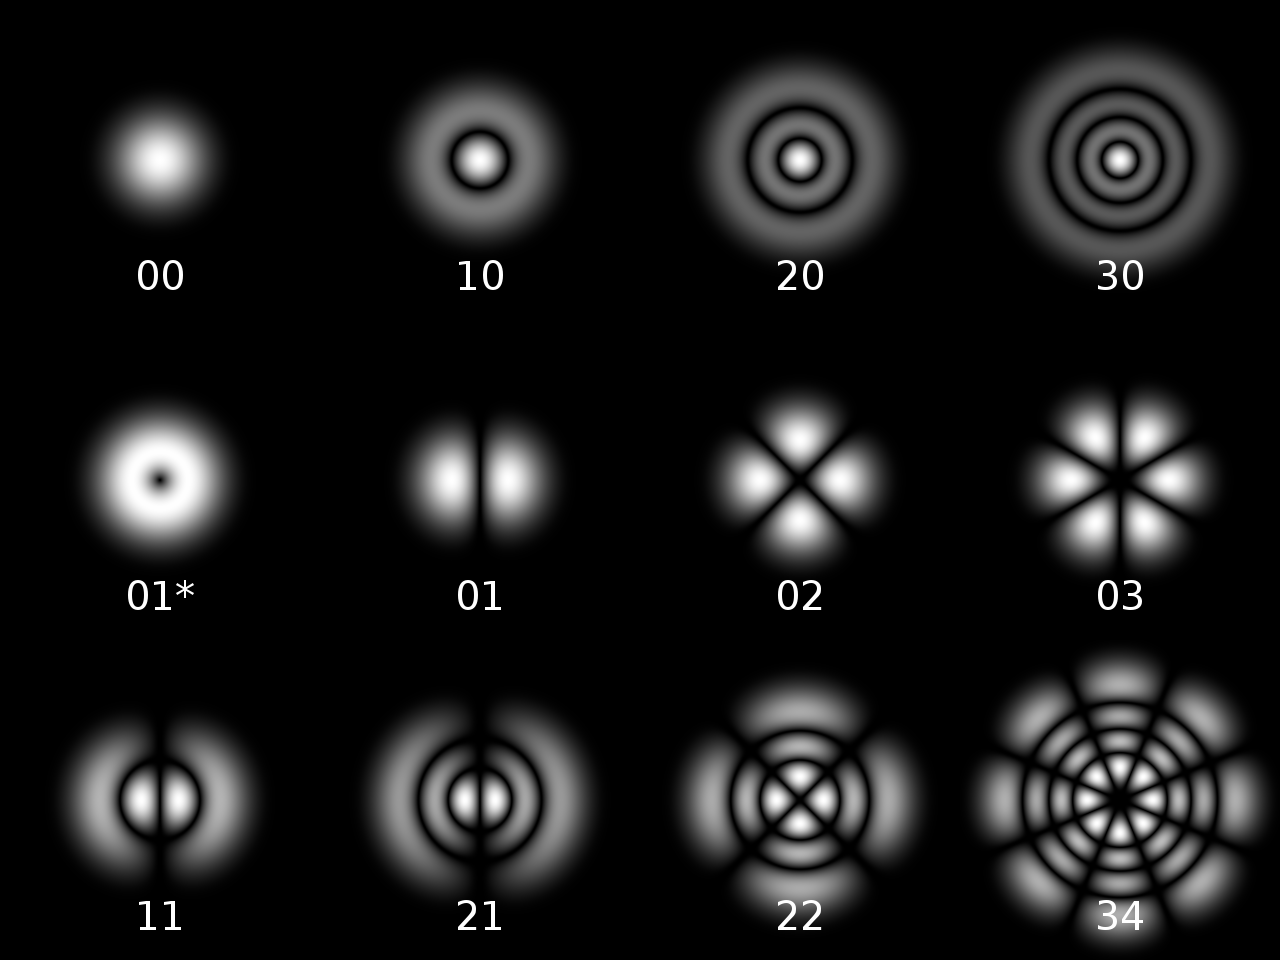
\includegraphics[width=3.2in]{./Pictures/Laguerre-gaussian.png}
\caption{\label{fig:laguerre_modes}Laguerre-Gaussian resonator modes for an optical cavity. Figure courtesy of {\it Wikimedia Commons}.}
\end{center}
\end{figure}

Mode-matching the laser to the fundamental TEM$_{00}$ mode requires matching the radius of curvature $R_M(z)$ (equation \ref{eq:R_m}) to the radius of curvature of the mirrors in the optical cavity. This is illustrated in Figure \ref{fig:mode_matching}. The better mode-matched a laser is to an optical cavity, the more power will be coupled into the fundamental cavity oscillating mode and the less will be reflected backward. The Gaussian fundamental mode is matched to the cavity by finding lens positions that create the beam radius of curvature $R_M$ that matches the radius of curvature of the cavity mirrors.

\begin{figure}
\begin{center}
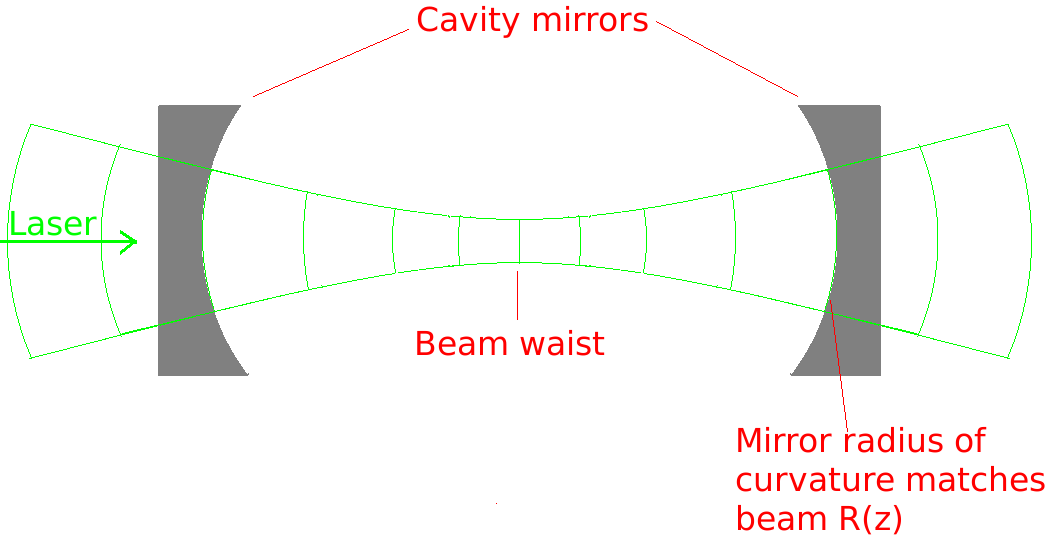
\includegraphics[width=4in]{./Pictures/mode_matching}
\end{center}
\caption{\label{fig:mode_matching}Illustration of symmetric optical cavity mode-matched to TEM$_{00}$ mode of laser. The laser wavefront radius of curvature is matched to the surface of cavity mirrors.}
\end{figure}

Before an optimal mode-matching solution can be found, the laser's propagation equations, $w_M(z)$ and $R_M(z)$, must be determined. Measurements of the beam profile as a function of $z$ allows one to fit $w_M(z)$ to determine the parameters $w_{0M}$ and $M^2$, which are sufficient to fully define Equations \ref{eq:w_m} and \ref{eq:R_m}. Beam profile measurements on the Compton laser were performed using a camera for imaging the transverse dimensions of the beam, with software for calculating estimates of the beam radius\footnote{The beam was not actually assumed to be circular. The software determined beam widths for the two transverse dimensions of the beam.}. The camera was moved along the beam in discrete steps to measure the profile as a function of $z$. Measurements were taken on both sides of a waist and extended to the far-field region where the beam divergence is nearly linear in $z$. These measurements were then used to find the laser propagation equations. A linear optics model with the system described in terms of matrices\cite{Kogelnik}, was then used to determine the optimal positions for a given set of lenses to produce the desired beam shape matched to the optical cavity. Figure \ref{fig:mode_match} shows an example of a particular solution used on the Hall C Compton laser table. 

\begin{figure}[h]
\begin{center}
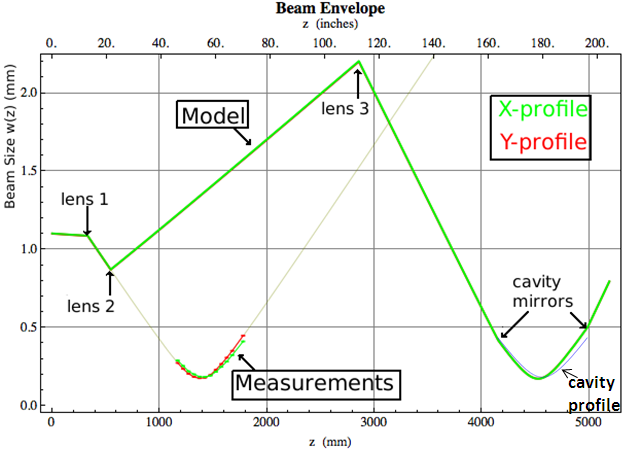
\includegraphics[width=5in]{./Pictures/HallC_mode_match_cavity_profile.PNG}
\end{center}
\caption{\label{fig:mode_match}Laser size as a function of $z$ along its path. To mode-match the laser to the optical cavity careful measurements were taken around the waist with only lens 1 installed. Notice that X and Y profiles do not have a waist at the same z-location. Fitting these measurements yields $w_M(z)$ and $R_M(z)$ which are then fed to an optimization routine for determining the best locations for lenses 2 and 3. The cavity TEM$_{00}$-mode profile for mirrors with radius of curvature $R=50$~cm and laser $w_{0M}=184~\mu$m is also shown, indicating a small mismatch with the predicted laser profile. }
\end{figure}
 
In order to build up power in a Fabry-Perot optical cavity, the length of the cavity must be an integer number of wavelengths of the incident light. This condition, called the resonance condition for constructive interference, can be expressed as
\[
 2L=n\lambda,
\]
where $L$ is the cavity length, $\lambda$ is the wavelength of the light and $n=1,2,3...$ is an integer greater than zero. With a wavelength of 532~nm, small vibrations are sufficient to take a macroscopic optical cavity in and out of resonance, requiring a continuous feedback on either cavity length or on laser wavelength to maintain the resonance condition. The Verdi V-10 laser was retro-fitted with actuators to allow fine adjustment of the laser wavelength around the 532~nm mean. This was accomplished by mounting one of the internal resonator mirrors on two stacks of piezo-electric (PZT) material\cite{Coherent}. A short stack with low inertial mass was used for small cavity length changes at frequencies up to 20~kHz, typically associated with corrections for acoustic noise. A tall stack enabled larger mirror displacements to correct for slow drifts such as thermal changes. Both the slow and fast channels were adjusted with independent PID feedback loops with outputs in the 0-100~V range. Figure \ref{fig:lockedcavity} shows a picture of a Fabry-Perot optical cavity locked on the cavity resonant frequency during the research phase at the University of Virginia.

\begin{figure}
\begin{center}
  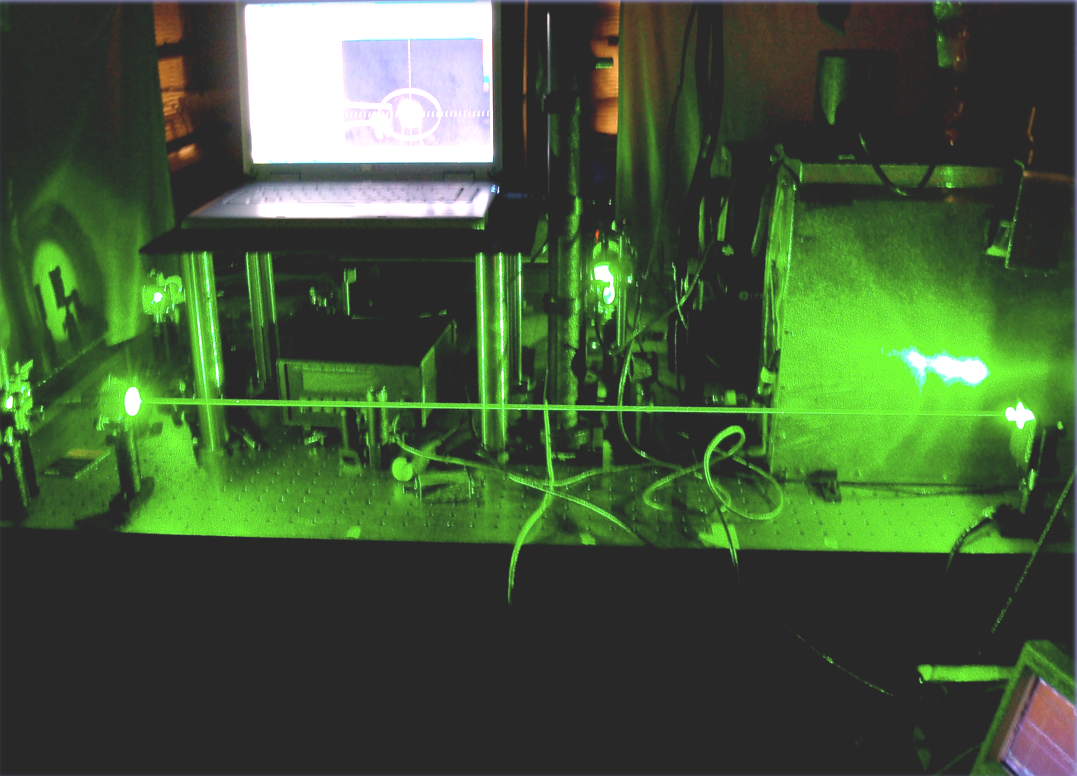
\includegraphics[width=4in]{./Pictures/lockedcavity.PNG}
\caption{Locked optical cavity shown during testing on an optics table at the University of Virginia. During the research phase shown, cavity lock was maintained by feeding back on the external cavity length. Cavity length was changed by attaching one of the cavity mirrors to a PZT stack. }
\label{fig:lockedcavity}
\end{center}
\end{figure}

The feedback signal for maintaining cavity resonance was created using the Pound-Drever-Hall (PDH) technique for frequency stabilization. The setup for this technique is illustrated in Figure \ref{fig:PDH_setup}. For the Hall C Compton, the technique was employed as follows. The laser was phase-modulated at 6.25~MHz using an electro-optical modulator (EOM). The EOM served as the capacitor in an oscillating resistor-capacitor (RC) circuit, tuned to resonate at 6.25~MHz\footnote{Phase-modulating the light produces a frequency distribution with most of the power near the main laser frequency and a small fraction in ``sidebands'' at the sum and difference of the laser and modulation frequencies. Near resonance these sidebands are reflected from the cavity since they are far from the resonance condition. The interference between these sidebands and the central laser frequency is used to produce the error signal for feeding back on laser wavelength to maintain cavity lock. Although a detailed analysis of the PDH locking technique is beyond the scope of this discussion, a conceptual overview can be found at \cite{Black}.}. The modulated light then passed through a polarizing beam splitter and quarter wave plate oriented to produce circularly polarized light. Circularly polarized light reflected from the entrance cavity mirror was deflected by the polarizing beam splitter into a photodiode termed the reflected photodiode (RPD). The signal from the RPD was then mixed with a phase-adjusted oscillator frequency for demodulation, producing sum and difference frequencies. The difference frequency (difference between the oscillator and RPD) produces a DC signal approximately proportional to the frequency offset from resonance for small offsets. This comparatively low frequency signal is filtered out using a low pass filter and then amplified and used as the error signal for a PID feedback loop connected to the laser frequency adjustment actuators. A general purpose, digital locking module, the Digilock 110 Feedback Controlyzer built by Toptica Photonics, was used to maintain cavity lock and greatly simplified the laser locking setup, providing a method for remote control of the electronics. Details on the Digilock module can be found in \cite{Digilock}. 
\begin{figure}
\begin{center}
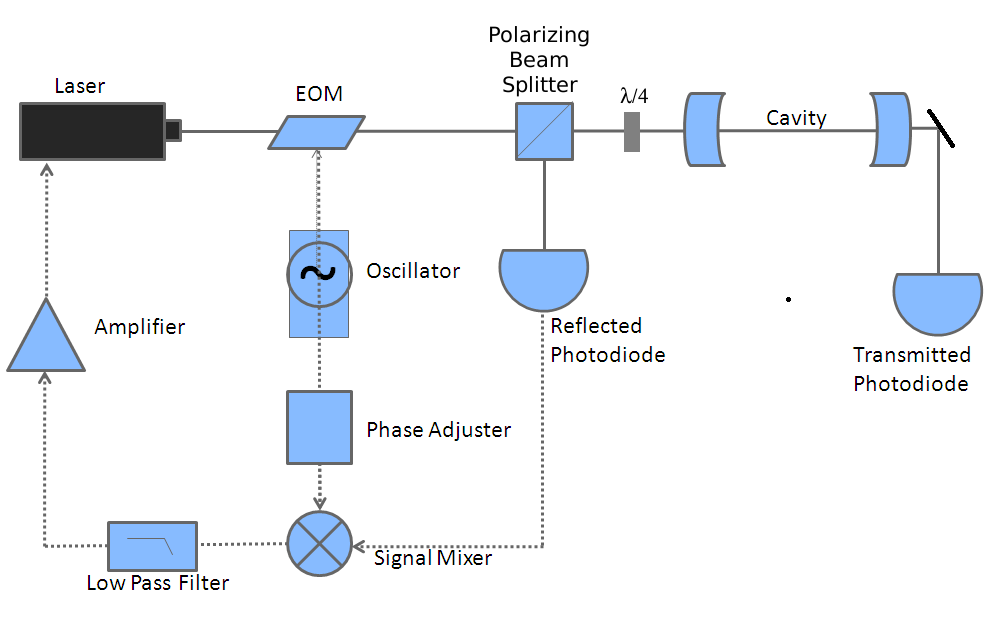
\includegraphics[width=5in]{./Pictures/PDH_setup.PNG}
\caption{Basic hardware setup for Pound-Drever-Hall cavity locking technique. Transmitted photodiode shown but not used in this setup.}
\label{fig:PDH_setup}
\end{center}
\end{figure}

Figure \ref{fig:PDH_signals} gives an example of the PDH error signal as a function of frequency offset from resonance clearly showing the approximately linear region near resonance. Near resonance the power in the reflected photodiode decreases steeply while the transmitted photodiode signal rises. For a lossless cavity the sum of the signals in the reflected and transmitted photodiodes is constant. Figure \ref{fig:PDH_digilock} shows actual signals measured with the Compton laser setup.

\begin{figure}
\begin{center}
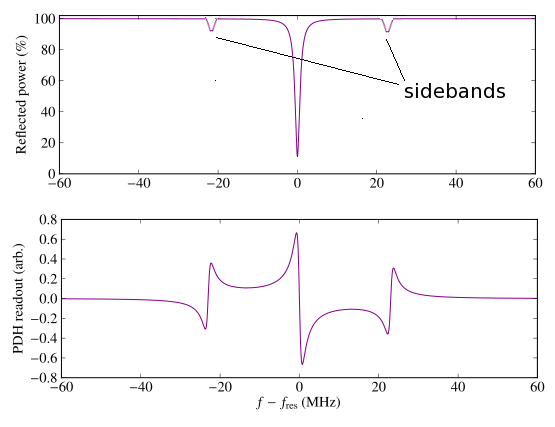
\includegraphics[width=4in]{./Pictures/PDH_signals_sidebands}
\caption{Curves drawn from expected functional form of PDH error signal and the readout from the reflected photodiode as a function of frequency offset from resonance. {\it Plots courtesy of Wikimedia Commons.} Plot edited to include exaggerated sidebands for purposes of illustration.}
\label{fig:PDH_signals}
\end{center}
\end{figure}

\begin{figure}
\begin{center}
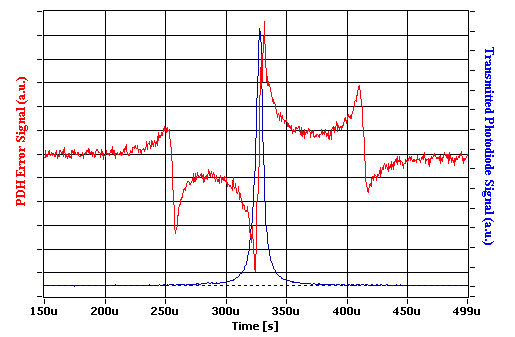
\includegraphics[width=4in]{./Pictures/PDH_error.PNG}
\caption{Digital trace of PDH error signals  and transmitted photodiode signal from Compton polarimeter laser electronics while scanning through resonance. Since the scan is a linear scan of the laser output wavelength, the horizontal time axis can also be thought of as frequency as in Figure \ref{fig:PDH_signals}. Notice that the transmitted signal is nearly the inverse of the reflected signal.}
\label{fig:PDH_digilock}
\end{center}
\end{figure}

The quality of cavity mirror alignment and laser mode-matching can be determined by the fraction of the light still detected in the reflected photodiode at resonance. A poorly aligned and/or mode-matched cavity may lock to cavity oscillating modes other than the TEM$_{00}$ mode where most of the laser power resides. In this case little power will be coupled into the cavity and most will be reflected. Even if the cavity is locked to the TEM$_{00}$ mode, the coupling of power into the cavity will be a function of the mode-match and alignment quality. During the \Qs experiment the mode-matching and cavity alignment were typically maintained to couple 60-80\% of the laser power into the cavity. The oscilloscope trace of the reflected photodiode signal seen in Figure \ref{fig:RPD_signal} demonstrates a configuration that yields 84\% power coupling.

\begin{figure}[!h]
\begin{center}
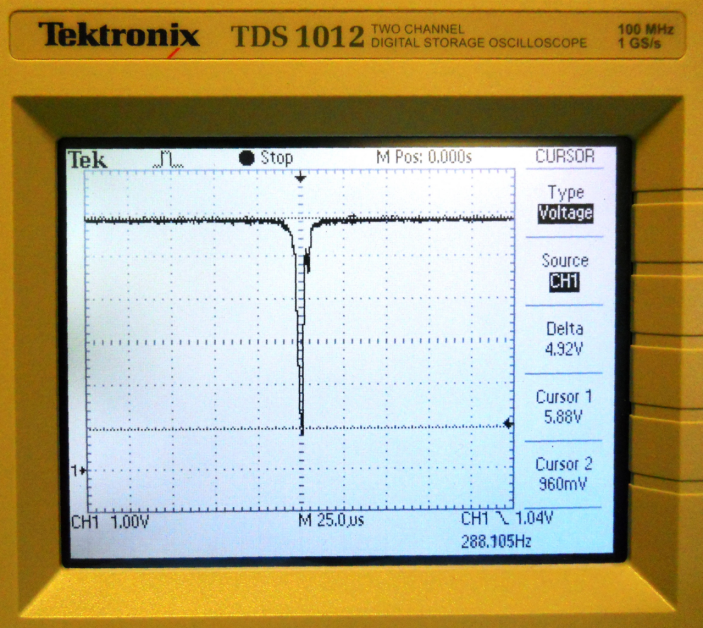
\includegraphics[width=3in]{./Pictures/RPD_signal.png}
\caption{Photograph of oscilloscope trace of reflected photodiode signal while scanning through resonance. Reading the cursor values printed on the screen to gauge the depth of the dip in the signal passing through resonance gives 4.92/5.88=84\% of the laser power coupled into the cavity.}
\label{fig:RPD_signal}
\end{center}
\end{figure}

The Fabry-Perot optical cavity for the Compton polarimeter was a symmetric design with both mirrors having a 50~cm radius of curvature, an overall cavity length of 84.2~cm and an electron beam crossing angle of $1.3^{\circ}$. This design produced a waist with a radius $w_{0M}$  of 180--190~$\mu$m at the center of the cavity\footnote{$w_{0M}$ is the radius that of the circular beam cross section that encloses $1/e^2$ of the laser power at its minimum size.}. High-reflectivity mirrors (R=99.5\%) yielded a cavity gain close to 200 with 1400--1800~W of stored power depending upon the quality of the mode-matching and laser alignment. Cavity finesse $\mathcal{F}$ is given by
\begin{equation}
\mathcal{F}=\frac{\pi}{2\sin^{-1}\left(\frac{1-R}{2\sqrt{R}}\right)}\approx \frac{\pi \sqrt{R}}{1-R}=627,
\end{equation}
for mirror reflectivity of 99.5\%. The cavity free spectral range, the frequency change between successive longitudinal resonant modes is given in terms of the cavity length $L$ as, $\nu_{fsr}=c/2L=178$~MHz. The cavity FHWM (full width at half maximum) linewidth, which is approximately the ratio of the free spectral range to the finesse, is $\Delta \nu_{_{FWHM}}=\frac{\nu_{fsr}}{\mathcal{F}}=284$~kHz.

 The electron beam optics were set up to have a much smaller electron beam spot size (1~$\sigma$ radius of 40~$\mu$m) at the point of interaction with the laser to avoid systematic errors associated with partial sampling of electron beam \footnote{It is possible to have polarization gradients across the cross section of the electron beam which could potentially bias polarization measurements. It would be useful to measure the sensitivity to the overlap of the laser and electron beams by taking polarization measurements with deliberately misaligned beams.}.  

Figure \ref{fig:tablelayout} shows a detailed diagram of the layout of the laser table with the individual components labeled. The laser emerged from the laser head primarily vertically polarized and was then dropped to 3 inches off the table by a periscope. It was then sent through an electro-optical modulator and two lenses used to shape it as seen in Figure \ref{fig:mode_match}. A half-wave plate followed by a horizontal linear polarizer both acted as a variable attenuator and rotated the beam polarization. Another shaping lens located 2 meters downstream provided the final matching before the cavity. After this lens the beam polarization was changed from linear to circular using a linear polarizer followed by a rotatable quarter-wave and a rotatable half-wave plate. A motorized periscope was then used to elevate and align the beam to enter the cavity inside the beam pipe. The beam arrived at the optical cavity and was partially reflected and partially transmitted. The reflected beam was deflected by the linear polarizer/polarizing beam splitter and was measured by the reflected photodiode attached to an integrating sphere. The transmitted beam was split and analyzed for power, position and polarization.

\newpage
\begin{figure}
\begin{center}
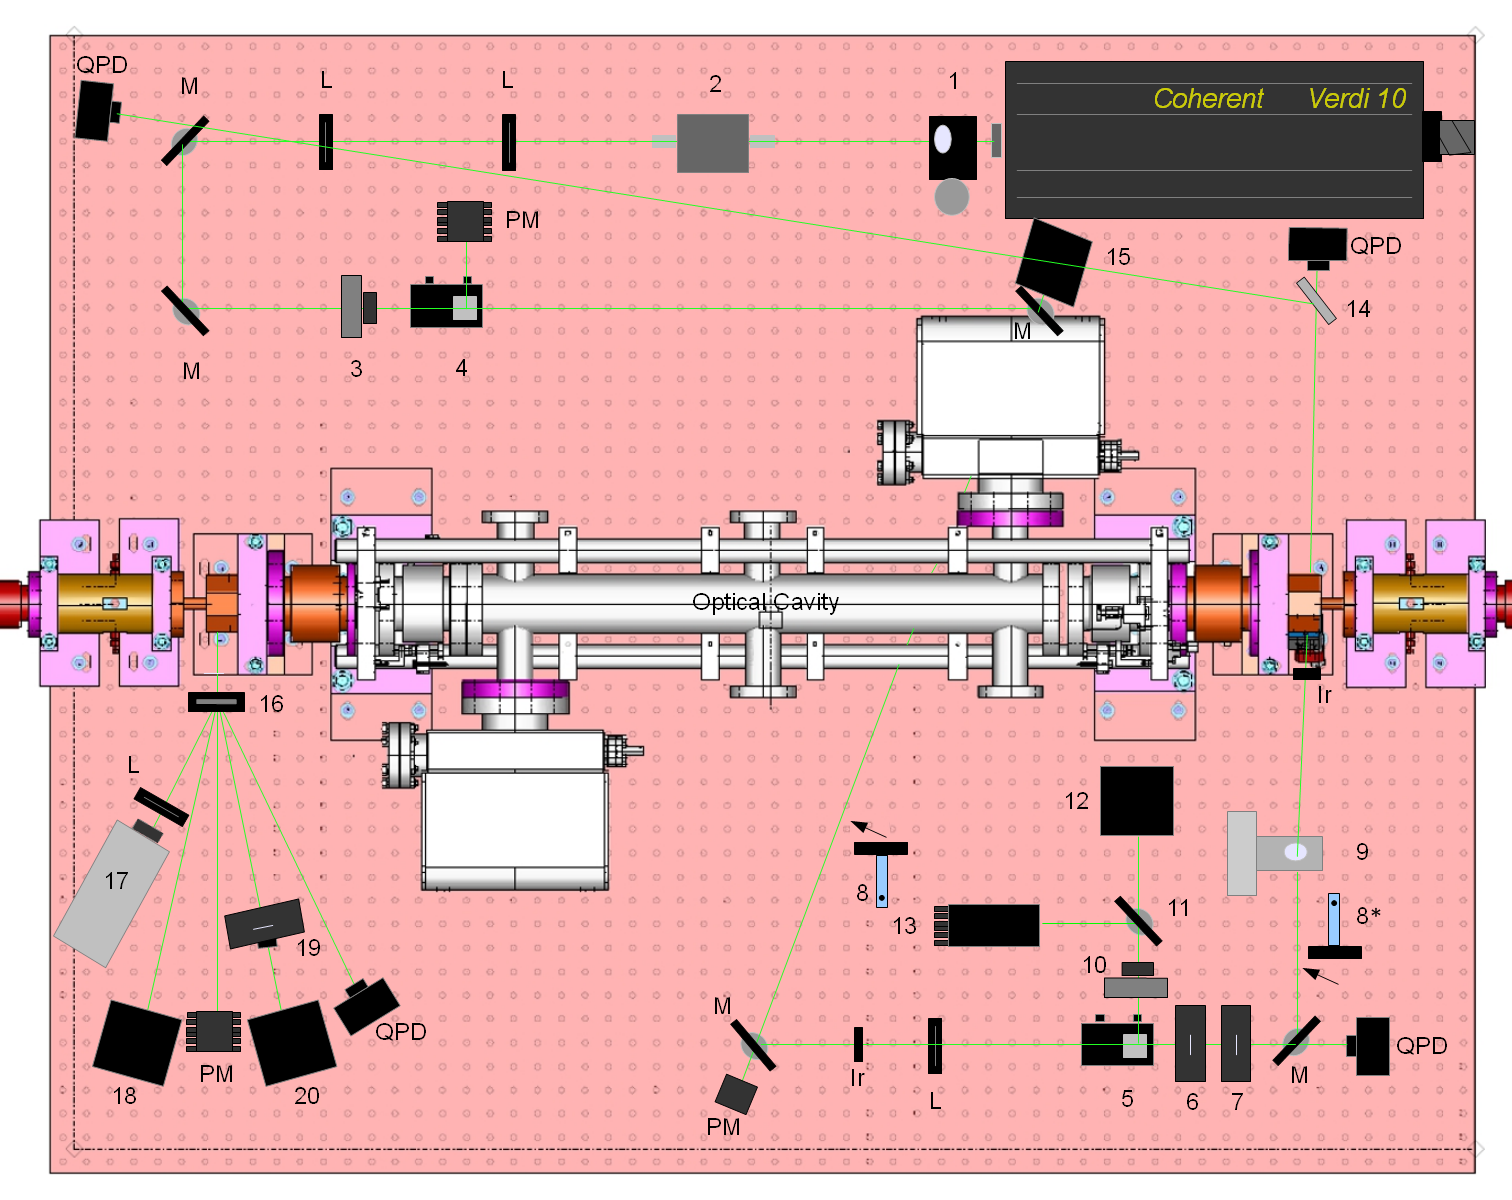
\includegraphics[width=6in]{./Pictures/tablelayoutwnmb.png}
\caption{Diagram showing a scaled version of the layout of the laser table and optical cavity overlayed by an engineering diagram of the electron beam pipe. Refer to the following list for component labeling.}
\label{fig:tablelayout}
\end{center}
\end{figure}
{\footnotesize{\noindent
QPD: quadrant photodiode to track laser position\\
L: lens for shaping beam\\
M: turning mirror\\
PM: power meter for monitor beam power\\
Ir: iris collimator (used only for setup and alignment of laser)\\
1. Manual periscope for dropping laser from 5 inch height at laser opening to 3 inches above table\\
2. EOM (electro-optical modulator) modulates frequency of laser at 6.25~MHz for Pound-Drever-Hall (PDH) cavity locking technique\\
3. Remote-controlled (RC) rotatable half wave plate. In conjunction with the polarizing cube at 4 we could control the fraction of laser power that was dumped into the power meter and the fraction that continued to the cavity.\\
4. Polarizing beam splitter. Here the vertically polarized light from the laser was changed to horizontally polarized.\\
5. Polarizing beam splitter. Creates horizontal linear polarization.\\
6. RC rotatable half-wave plate.\\
7. RC rotatable quarter-wave plate.  Combination of quarter and half wave plates allows one to tune the polarization to create perfect circular polarization at the cavity.\\
8. Flipper mirror inserted to block the beam during laser off times. This is the original position for most of Run 2. On March 16, 2012 the flipper was changed to position ``8*''.\\
9. RC periscope raises laser from 3 inches above the table to 9.5 inches above to the electron beam height.\\
10. Half wave plate used to adjust the fraction of light that goes through the partially reflecting mirror (11) into the Reflection Photodiode (12) and the fraction that is reflected into the beam dump (13).\\
11. Partially reflecting mirror (reflection coefficient sensitive to polarization state).\\
12. Reflection photodiode (RPD) attached to integrating sphere used to maintain cavity lock using PDH method.\\
13. High power beam dump.\\
14. 50\% beam splitter\\
15. Residual reflection photodiode (RRPD) attached to integrating sphere. Note that in this analysis the RRPD is referred to as the ``leakage photodiode''. Monitors component of light that is reflected off the cavity mirror and back through the linear polarizer (5). Adjusting the HWP(6) and QWP(7) to minimize the light in the photodiode (15) maximizes the degree of circular polarization at the optical cavity.\\
16. Holographic beam splitter (HBS) splits the beam into several beam approximately 17 degrees apart. The main beam carries about 98\% of the power with the first order beams on either side having 1\% each and the second order beams a very small fraction.\\
17. LCD camera for viewing transmitted beam. Used for imaging transmitted beam on screen in counting house.\\
18. Transmitted photodiode monitors relative power of transmitted beam and thus the power stored in the cavity.\\
19. RC rotatable Glan Laser linear polarizer.\\
20. Transmitted photodiode. The degree of linear polarization (DOLP) of the transmitted beam was measured by rotating the linear polarizer and measuring the photodiode signal as a function of rotation angle. This signal was normalized to the power in (18) to remove laser and cavity power fluctuations. DOLP=amplitude/offset of sine fit to signal vs angle.\\}
}
\section{Laser Polarization}
This section is devoted to determining the polarization of the photon target and will be divided into two topics. The details of the theory and methods used in determining the laser polarization inside the optical cavity will be first developed including difficulties encountered. Second, these methods will be applied to the Compton polarimeter dataset for Run 2 of \Qs to provide the laser polarization and assign a systematic error.
\subsection{\label{Sctn:Methodology}Methodology and Theory} 
The Compton scattering asymmetry in equations \ref{eq:ameas} and \ref{eq:asymtopol} arises from a dependence on the electron and photon helicities in the scattering cross section. A beam of light with a single definite helicity is said to be circularly polarized. In terms of individual photons, this simply means the photons are either spin left or right. In terms of light as a wave, this means the electric field vector rotates about the axis of propagation. A circularly polarized laser has two perpendicular linearly polarized components of light that are out of phase by $90^{\circ}$ or $\pi/2$ wavelengths. It is this phase difference that causes the electric field to rotate in a continuous circle. By convention, a left(right)-hand spin photon (left(right)-circularly polarized light) is defined as clockwise(counterclockwise) spin when viewed with the light traveling directly toward the viewer.

In 1941 Robert Clark Jones wrote a series of three papers outlining a method for describing polarized light as a complex two-component vector, and optical systems with 2$\times$2 complex matrices \cite{Jones1}\cite{Jones2}\cite{Jones3}. The Jones formulation for light propagation will be followed in the discussion ahead. Light is treated as a plane wave and since only electromagnetic fields transverse to the direction of travel are possible, the plane wave is expressed as a 2-vector:
\begin{equation}
\left[\begin{array}{c}E_xe^{i\phi_x}\\E_ye^{i\phi_y}\end{array}\right]e^{(kz-\omega t)},
\label{eq:jones_vector}
\end{equation}
where $E_{x(y)}$ are the amplitudes of the electromagnetic wave in the x (y) directions, $\phi_{x(y)}$ are the phases of the plane wave in the x (y) directions and $k$ and $\omega$ are the wavenumber and frequency of the light respectively. Since only the relative phase is measurable this equation can be further simplified to
\begin{equation}
\left[\begin{array}{c}E_x\\E_ye^{i\phi}\end{array}\right],
\label{eq:jones_vector_simple}
\end{equation}
where $\phi$ is the relative phase $\phi_y-\phi_x$ and the overall wave propagation term has been removed. Table \ref{tab:jones_vectors} gives examples of some common polarization states using Jones vectors. 
\begin{table}
\caption{\label{tab:jones_vectors}States of light polarization using Jones vectors. All vectors normalized to unity.}
\begin{center}
\begin{tabular}{|l|c|}\hline
Horizontal linear polarization&$\left(\begin{array}{c}1\\0\end{array}\right)$\\\hline
Vertical linear polarization&$\left(\begin{array}{c}0\\1\end{array}\right)$\\\hline
Right circular polarization&$\frac{1}{\sqrt{2}}\left(\begin{array}{c}1\\-i\end{array}\right)$\\\hline
Left circular polarization&$\frac{1}{\sqrt{2}}\left(\begin{array}{c}1\\i\end{array}\right)$\\\hline
\end{tabular}
\end{center}
\end{table}
Jones vectors are manipulated using 2$\times$2 matrices representing optical components. The effect of multiple optical elements is given by matrix multiplication of the respective elements in the order in which they are encountered by the ray of light. The matrix representations of a few common optical elements are shown in Table \ref{tab:jones_matrices}. Some of these elements are special cases of the basic optical elements. For example, the horizontal polarizer is a special case of the partial polarizer with $p_x=1$, $p_y=0$ and circular polarizers are special cases of phase retarders with $\gamma=\pi/4$ and with the birefringent axis rotated $\pm 45^{\circ}$ with respect to the horizontal axis. 
\begin{table}
\caption{\label{tab:jones_matrices}Matrix representations for some common optical components in the Jones formulation. The partial polarizer and phase retarder are shown with their extinction and retardance axes respectively lined up along the vertical and horizontal axes of the coordinate system.}
\begin{center}
\begin{tabular}{|l|c|c|}\hline
Element&Symbol&Matrix Representation\\\hline
Horizontal linear polarizer&$\bf P_x$&$\left(\begin{array}{c c}1&0\\0&0\end{array}\right)$\\\hline
Vertical linear polarizer&$\bf P_Y$&$\left(\begin{array}{c c}0&0\\0&1\end{array}\right)$\\\hline
Right circular polarizer&$\bf P_R$&$\frac{1}{2}\left(\begin{array}{c c}1&i\\-i&1\end{array}\right)$\\\hline
Left circular polarizer&$\bf P_L$&$\frac{1}{2}\left(\begin{array}{c c}1&-i\\i&1\end{array}\right)$\\\hline
Partial polarizer&$\bf P$&$\left(\begin{array}{c c}p_x&0\\0&p_y\end{array}\right),0\ge p_{x,y}\le1$\\\hline
Linear polarization rotator&$\bf S(\omega)$&$\left(\begin{array}{c c}\cos{\omega}&-\sin{\omega}\\\sin{\omega}&\cos{\omega}\end{array}\right)$\\\hline
Phase retarder&$\bf G(\gamma)$&$\left(\begin{array}{c c}e^{i\gamma}&0\\0&e^{-i\gamma}\end{array}\right)$\\\hline
Mirror (normal incidence)&$\bf M$&$\left(\begin{array}{c c}-1&0\\0&1\end{array}\right)$\\\hline
\end{tabular}
\end{center}
\end{table}

In general, perfectly reflecting  mirror at non-normal incidence will have different phase shifts for the polarization states perpendicular and those parallel to the plane of incidence, called the $s$ and $p$ polarizations respectively and can be modeled as an arbitrarily rotated birefringent element (phase retarder) taking the form ${\bf S(\omega)G(\gamma)S(-\omega)}$ \cite{Vansteenkiste}. If one adds to this an arbitrarily-oriented, stress-induced birefringence on the mirror surface, two independent rotation matrices are required as follows: ${\bf S(\omega_1)G(\gamma)S(-\omega_2)}$. This simple form can be extended to include any optical system composed of combinations of polarization rotators and phase retarders (which includes lossless mirrors). These lossless optical systems can be modeled using a single phase retarder with retardance axes aligned along the x and y axes of the coordinate system sandwiched between two rotation matrices as follows (Equation 4 \cite{Jones2}):
\begin{equation}
{\bf S(\omega_2)G(\gamma)S(\omega_1)},
\label{eq:simple_optics}
\end{equation} 
where $\omega_1$ and $\omega_2$ are not in general equal. 

All matrices in this model are unitary. Thus, in this simple model vector length is conserved and no light is lost or absorbed. Polarizing optics do not necessarily conserve light intensity and are, therefore, represented by non-unitary matrices. Optical systems composed of any arrangement of phase retarders, rotators and polarizers can be modeled by a partial polarizer sandwiched between two phase retarders and a rotator added anywhere in the system (see equations 23, 24 in \cite{Jones2}). For the purposes of this study, however, it will be sufficient to include only lossless optical elements (rotators and birefringent plates). This statement will be justified where necessary in the ensuing discussion.  

\begin{figure}[ht]
\centering
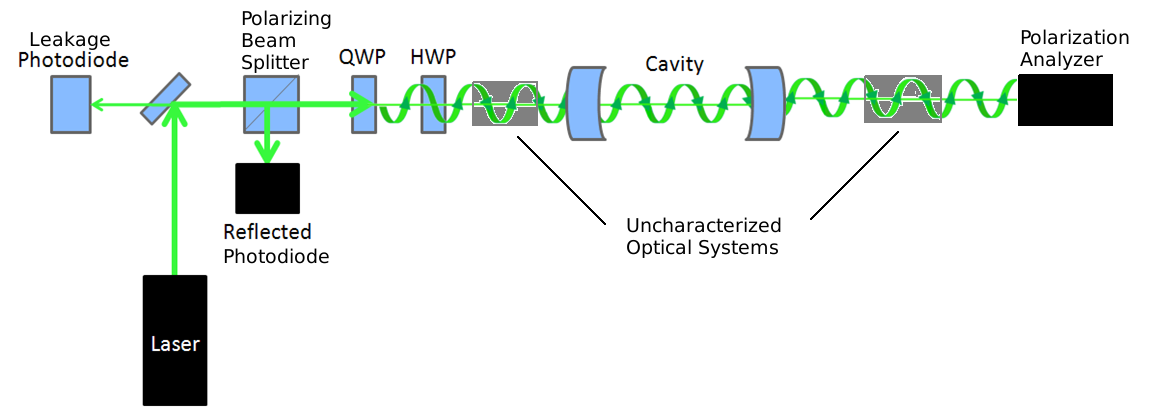
\includegraphics[width=5.5in]{./Pictures/optical_schematic.png}
\caption{\label{fig:optical_schematic}Simplified schematic of optical setup for producing and measuring polarized light inside Fabry-Perot optical cavity.}
\end{figure}

The use of a locked optical cavity as a photon target, together with its placement inside the high-vacuum region of the electron beam enclosure, creates challenges for determination of laser polarization. High losses, steering, and birefringence associated with analyzing optical components make it impossible to directly measure the light inside the cavity. However, in principle, both the reflected and transmitted beams can be analyzed to infer the polarization inside the cavity. Figure \ref{fig:optical_schematic} shows a simple schematic of the optical setup used to produce the photon target. Notice the regions before and after the optical cavity labeled ``uncharacterized''. These regions each have turning mirrors and a vacuum window. The transmitted region also has a holographic beam sampler for splitting the transmitted laser into several beams of different power levels. If the entrance (exit) optical system were fully characterized one could determine the polarization inside the cavity by measuring the polarization characteristics (ellipticity and angle of the polarization ellipse) of the reflected (transmitted) beam. 

Near the beginning of \Q, an attempt was made to characterize the exit region optics to infer laser polarization inside the cavity from exit line measurements of laser polarization. This process involved disassembling the cavity region of the beam pipe and installing optical components inside the optical cavity. A set of polarization states were set up and carefully measured in the optical cavity region. These same states were then measured with the polarization analyzer in the exit line region. Assuming that the optical elements can be modeled as a series of lossless mirrors, arbitrarily rotated birefringent plates and polarization rotators, this optical system can be characterized by three degrees of freedom as given in Equation \ref{eq:simple_optics}. In this setup only beam polarization characteristics are being measured, not absolute beam power. Therefore, this model is also valid for lossy optical components as long as they are not polarization-dependent losses. Fitting for the three parameters in this model, two rotation angles ($\omega_{1}$ and $\omega_{2}$) and one birefringence phase shift ($\gamma$) produces gives an optical system matrix called the transfer function ({\bf TF}) which tells how the polarization evolves from the second mirror of the optical cavity to where it can be measured in the exit line polarization analyzer. This fit involves minimizing the quadrature difference in the degree of circular polarization measured in the exit region and that predicted by the optical transfer matrix. Measurements in the exit line polarization analyzer can be translated into intra-cavity polarizations as follows:
\[
\bf E^{exit}=(TF)E_{cavity}\longrightarrow E_{cavity}=(TF)^{-1}E_{exit},
\]
where ${\bf E_{exit}}$ and ${\bf E_{cavity}}$ are the Jones vectors representing the polarization state of the laser in the cavity and where it is measured in the exit line respectively. 

Although one might be tempted to question the validity of the simple model given the known polarization-dependent reflectivities of typical mirrors, a more outstanding problem with this method arises from stress-dependent birefringence in the vacuum windows. A set of measurements taken during the break between Runs 1 and 2 of the \Qs experiment showed evidence that the transfer matrix depended upon the stress placed on the vacuum window. The main factors that affected the birefringence of the windows were temperature, vacuum pressure and bolt tensioning on the beam pipe components near the windows. The plot in Figure \ref{fig:TF_change} shows how the polarization of the laser measured in the exit line changed as the beam pipe in the optical cavity region was reassembled and vacuum was pulled, implying that the transfer matrix measured with the cavity region disassembled was not the same as the required transfer matrix of the fully reassembled system under high vacuum. 

\begin{figure}[ht]
\centering
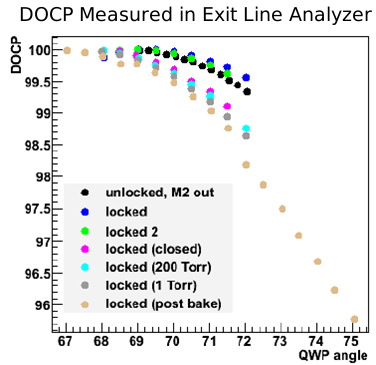
\includegraphics[width=4in]{./Pictures/ChangingTF.png}
\caption{\label{fig:TF_change}Degree of circular polarization (DOCP) measured in the exit line as a function of input quarter-wave plate angle. The input state as given by the quarter-wave plate (QWP) angle that produced maximum exit DOCP had to be adjusted by several degrees as modifications (tensioning bolts, pulling vacuum, baking) were made to the cavity. The legend can be interpreted as: 1. ``unlocked, M2 out''--second cavity mirror removed 2. ``locked''--optical cavity locked during measurement 3. ``locked 2''--second measurement with optical cavity locked 4. ``locked (closed)'' cavity region reassembled and bolts tensioned 5. ``locked (200~Torr)''--vacuum pulled to 200~Torr and cavity locked 6. ``locked (1~Torr)''-- vacuum pulled to 1~Torr and cavity locked 7. ``locked (post bake)''-- cavity locked after optical cavity baked producing high vacuum. The QWP setting for maximum intracavity polarization post bake was between 72$^{\circ}$ and 73$^{\circ}$.}
\end{figure}
 
Analysis of the entrance region optics presents a potential method for circumventing the unknown changes introduced by the vacuum window birefringence. The advantage of characterizing the entrance over the exit line optics is rooted in the fact that the light passes twice through the same system (forward and reverse) and under certain conditions comparison of the changes in the polarization states between the two beams provides sufficient information to characterize the intermediate optical system. This means that the optical transfer matrix for the entrance can be found without disassembling the cavity or breaking vacuum. Although it is satisfying to be able to properly model the optics of the system by building a transfer matrix, it will be shown that this is not strictly necessary and that maximum circular polarization at the cavity can be achieved without knowledge of the intermediate optical system. It is instructive, however, to demonstrate the possibility of creating an optical model by analysis of the reflected beam only.

Once again consider an optical model of birefringent plates, mirrors and rotators, all of which are either lossless or have polarization-independent losses, as a model for the uncharacterized optics at the entrance region of the cavity in Figure \ref{fig:optical_schematic}. The uncharacterized optics can be modeled by two rotators and a single birefringent plate as in Equation \ref{eq:simple_optics}. The QWP and HWP shown are rotatable and are directly introduced into the model but are not assumed to be perfect. Unknown birefringence errors on these plates are allowed in the model as are arbitrary rotation offsets of the optical axes. If the coordinate system is assumed constant no matter which direction the light propagates (forward or reverse), the optical system matrix for the returning light is simply the transpose of the forward system matrix. Thus the optics model has six fit parameters: two offsets for the waveplates, two errors for the waveplate birefringences and an arbitrary birefringence at an unknown rotation angle. Notice (Figure \ref{fig:optical_schematic}) that the incoming light passes through a linear polarizer (polarizing beam splitter) and the reflected light is analyzed by the same polarizer into its two linear states. The ``reflected photodiode''(labeled 12 in Figure \ref{fig:tablelayout}) and ``leakage photodiode'' (labeled 15 in Figure \ref{fig:tablelayout}) measure the intensity in the vertical and horizontal polarization states respectively. These photodiodes produce the signal measured to determine the output polarization state, that is, the Jones vector of the reflected light. The entrance function model matrix ${\bf M}$ is then
\begin{equation}
\begin{array}{lcl}
{\bf M}&=&\left[M_{element}(\alpha_0,\alpha_1)\right]\left[M_{HWP}(\alpha_2,\alpha_3)\right]\left[M_{QWP}(\alpha_4,\alpha_5)\right],\\
\text{with}&~&~\\
M_{element}&=&{\bf S}(\alpha_0){\bf G}(\alpha_1){\bf S}(-\alpha_0)\\
M_{HWP}&=&{\bf S}(\theta_{\frac{\lambda}{2}}\times\alpha_2){\bf G}(\pi/2 +\alpha_3){\bf S}(-\theta_{\frac{\lambda}{2}}\times\alpha_2)\\
M_{QWP}&=&{\bf S}(\theta_{\frac{\lambda}{4}}\times\alpha_4){\bf G}(\pi/4 +\alpha_5){\bf S}(-\theta_{\frac{\lambda}{4}}\times\alpha_4),\end{array}
\end{equation}
where the $\alpha_i's$ are fit parameters, $\theta_{\frac{\lambda}{2}(\frac{\lambda}{4})}$ are the rotation angles of the half(quarter)-waveplates and the matrices are defined in Table \ref{tab:jones_matrices}. If one chooses to use the same coordinate system for the optical system regardless of the direction of the light, the optical matrix for the returning beam is simply the transpose of ${\bf M}$ (Equation 11 \cite{Vansteenkiste}). Analysis of the reflected beam requires no additional degrees of freedom. The output measured in the two photodiodes is then given as
\begin{equation}
\left[\begin{array}{c}a_0(PD-p_0)_{Leakage}\\a_1(PD-p1)_{Reflected}\end{array}\right]={\bf M^T M}\left[\begin{array}{c}1\\0\end{array}\right],
\label{eq:entrance_model}
\end{equation}
where $(PD-p)$ are the pedestal subtracted signals in the two photodiodes and $a_{0,1}$ are the normalization constants. The initial state $\left[\begin{array}{c}1\\0\end{array}\right]$ shows that the initial state of the laser before entering the optical setup is horizontally polarized. The leakage photodiode measures the returning horizontally polarized component of the reflected beam and the reflected photodiode measures the vertically polarized component. Both the pedestals $p_{0,1}$ and the normalization constants $a_{0,1}$ are included as fit parameters since the photodiode signals are not absolute power measurements, bringing the total number of fit parameters to 8.

To determine the parameters of the model a full scan of the half-wave and quarter-wave plates was done and the signals in the photodiodes measured as a function of the rotation angle. Although data from either of the photodiodes is sufficient to obtain the parameters of the model, scans were taken of both the leakage and reflected photodiodes. Fits were performed to find the best parameters of the model using MINUIT to minimize the square of the difference between the signals measured in the photodiodes and that predicted by the model\footnote{More accurately the square of the difference normalized to the estimated variance of the difference was minimized. This is just a $\chi^2$ minimization.}.  The model parameters found separately using the data from the two photodiodes are given in Table \ref{tab:minuit_params} and show excellent agreement. 
\begin{table}[ht]
\caption{\label{tab:minuit_params}Model parameters from fit to signals measured in the reflected and leakage photodiodes during a scan of quarter-wave and half-wave plates.}
\begin{tabular}{l|c|c|c|c}
Description&Name&Leakage PD& Reflected PD&Units\\\hline
Pedestal&$p_{0,1}$&$32831.8\pm0.3$&$32749.8\pm0.3$& arb\\
Power normalization&$a_{0,1}$&$2486.4\pm0.6$&$894.4\pm0.5$& arb\\
Birefringence angle&$\alpha_0$&$-2.2980\pm0.0004$&$-2.29\pm0.01$& degrees\\
Birefringence phase&$\alpha_1$&$-0.1051\pm0.0001$&$-0.1048\pm0.0002$& radians\\
$\lambda/2$ plate rotation offset&$\alpha_2$&$78.784\pm0.002$ &$79.2\pm0.3$& degrees\\
$\lambda/2$ plate phase error&$\alpha_3$&$0.9671\pm0.0002$&$0.9652\pm0.0004$&fractional\\
$\lambda/4$ plate rotation offset&$\alpha_4$&$43.516\pm0.003$&$44.1\pm0.6$&degrees\\
$\lambda/4$ plate phase error&$\alpha_5$&$1.0141\pm0.0002$&$1.0117\pm0.0006$&fractional\\
\end{tabular}
\end{table}

Figures \ref{fig:RRPD_scan} shows the measured leakage photodiode signal along with the model predictions (model parameters taken from MINUIT fit) as function of quarter and half-wave plate positions. The model appears to accurately reproduce the measured power in the photodiode. A similar pair of plots is provided for the reflected photodiode in Figure \ref{fig:RPD_scan}. The reflected and leakage photodiodes show similar patterns with the the minimum signal in the reflected occurring at the maximum of the leakage and vice versa. 
\begin{figure}
\centering
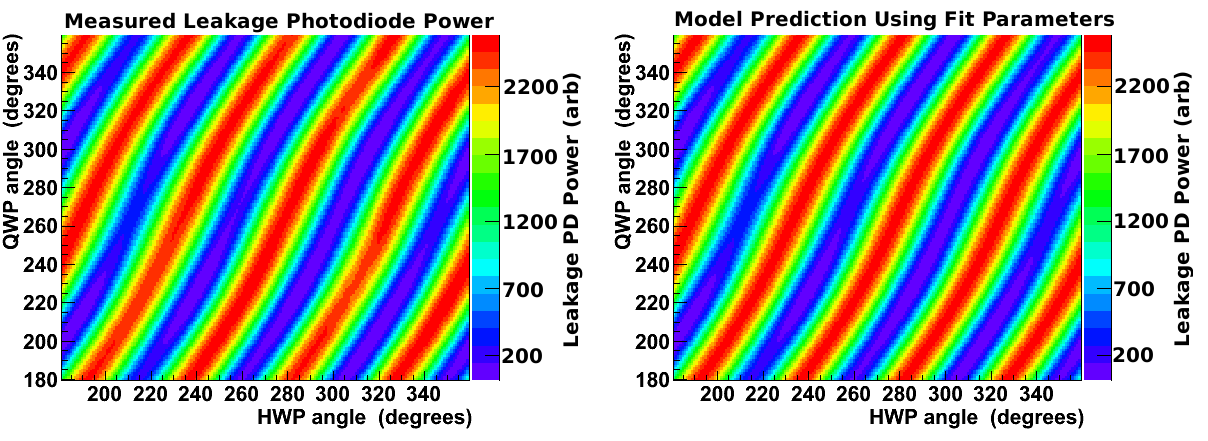
\includegraphics[width=5.6in]{./Pictures/RRPD_scan.png}
\caption{\label{fig:RRPD_scan}Leakage photodiode signal as a function of half-wave and quarter-wave plate rotation angle. Measured signal shown on the left and prediction from model (Equation \ref{eq:entrance_model}) using fit parameters in Table \ref{tab:minuit_params}.}
\end{figure}

\begin{figure}
\centering
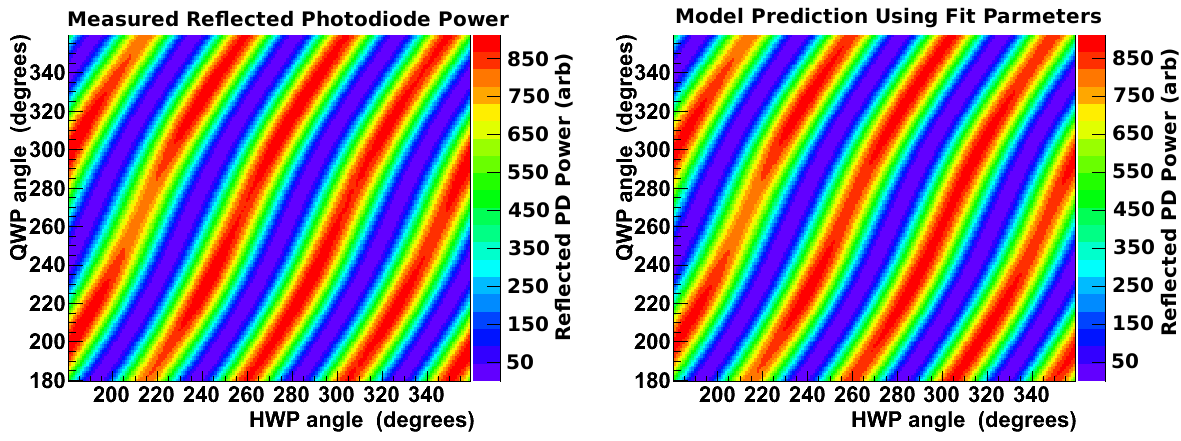
\includegraphics[width=5.6in]{./Pictures/RPD_scan.png}
\caption{\label{fig:RPD_scan}Reflected photodiode signal as a function of half-wave and quarter-wave plate rotation angle. Measured signal shown on the left and prediction from model (Equation \ref{eq:entrance_model}) using fit parameters in Table \ref{tab:minuit_params}.}
\end{figure}

Figure \ref{fig:PD_residuals} shows the residuals, that is, the difference between the measured values and those predicted in the model, as a function of wave plate rotation angles. An ideal model has residuals that vary randomly around 0. The obvious structure in these residual plots show that there is something missing from the simple model. First, back-reflections off optical elements such as the quarter-wave and half-wave plates end up in the photodiodes. A better fit could be obtained if the beam were blocked after these elements and a full scan done to simply measure and subtract off the background (ambient light plus back-reflections) as a function of wave-plate angles. This is especially obvious in the vertical blue stripe apparent in the reflected photodiode residual and less so in the leakage photodiode residual. This stripe between (HWP angles 300 and 320 degrees) appears to be associated with the half-wave plate rotation angle and could be something as simple as a speck of dust on the wave plate surface. Structure that follows the striped features of the measured photodiode power plots is evidence of an imperfect model as opposed to a poorly measured background. In any case, if one neglects this systematically different region of the model, the range of residuals is only 4-6\% of the range of the photodiode powers. If the determination of polarization were dependent upon the absolute accuracy of the model, these details would be important and to ``nail down''. However, it can be shown that the circular polarization at the optical cavity can be accurately determined without a precise determination of the model. 

\begin{figure}[ht]
\centering
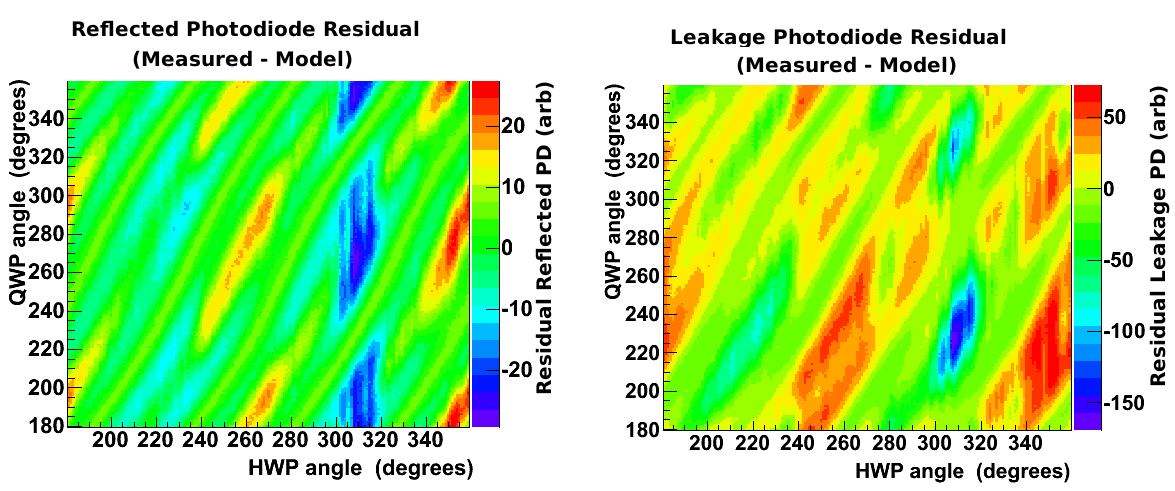
\includegraphics[width=5.6in]{./Pictures/Residual.png}
\caption{\label{fig:PD_residuals}Residuals (Measured Photodiode $-$ Model Prediction) for reflected (left) and leakage (right) photodiodes. The $3\times$ larger range of residuals in the leakage photodiode are mainly due to a $3\times$ larger overall signal size (compare maximum 900 channels in Figure \ref{fig:RPD_scan} and 2500 channels in Figure \ref{fig:RRPD_scan}).}
\end{figure}

Figure \ref{fig:DOCPvsRRPD} shows the DOCP obtained from the model at the entrance to the optical cavity as a function of quarter-wave and half-wave plate angles clearly demonstrating the ability of the setup to create any circular polarization state. Left and right helicity states are shown as -1 and +1 DOCP respectively. The strength of this model is not its ability to accurately predict DOCP, but the correlation that it shows between power measured in the photodiodes and the DOCP at the entrance to the optical cavity. The right plot in Figure \ref{fig:DOCPvsRRPD} shows the tight correlation predicted by the model for the leakage photodiode. A similar (but inverted parabola) correlation exits for the reflected photodiode but its usefulness as a measurement of polarization is reduced by the fact that its power is maximized at maximum DOCP and by its sensitivity to cavity power. The leakage photodiode has a minimum signal when the DOCP at the cavity entrance is maximized and near maximum DOCP its signal changes little with cavity lock quality making it a very sensitive parameter for adjusting DOCP. Of course, this correlation between cavity DOCP and photodiode power comes from a model that has already been shown to have 5\% residuals; however, a simple verification of the correlations between DOCP and the two photodiode powers is sufficient since one can then simply minimize leakage photodiode power to achieve maximum DOCP. Furthermore, if polarizations near the maximum 100\% DOCP are found to be achievable, the effect of small changes in linear polarization on the DOCP will be greatly suppressed.

\begin{figure}[ht]
\centering
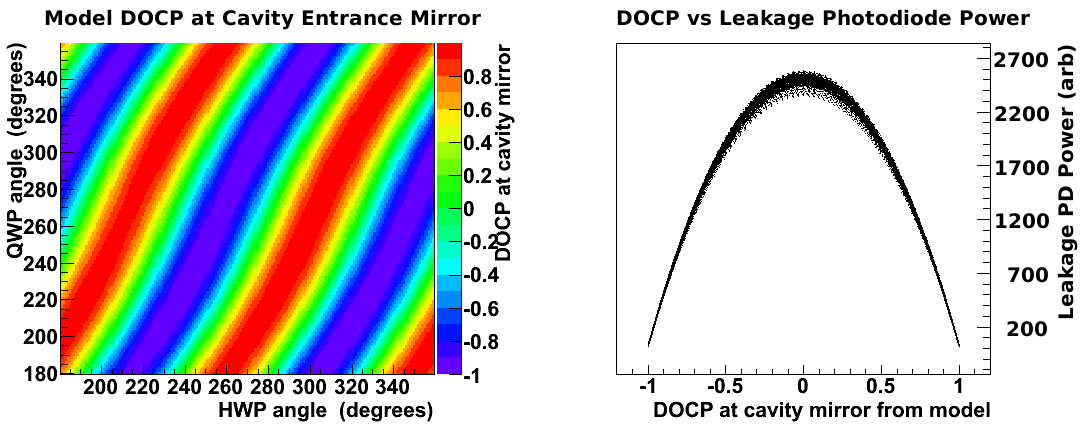
\includegraphics[width=5.6in]{./Pictures/DOCPvsRRPD.png}
\caption{\label{fig:DOCPvsRRPD}(Left) Degree of circular polarization  at entrance cavity mirror obtained from model as a function of quarter-wave and half-wave plate rotation angles. (Right)Model prediction of DOCP versus power measured in the leakage photodiode.}
\end{figure}

A series of measurements were taken with the cavity disassembled so that states inside the cavity could be directly measured albeit with the cavity unlocked. Figure \ref{fig:DOCP_measured_correl} shows the results of one such scan. The correlation of the cavity DOCP with the measured leakage photodiode power is confirmed and is shown to be approximately linear in the region near 100\% circular polarization. Figure \ref{fig:landr_docp_correl} shows a zoomed in region of the plot of DOCP versus leakage photodiode power clearly demonstrating the ability to reach 100.00\% circular polarization in both left and right circular states. Notice that the leakage photodiode signal is not 0 at 100\% circular polarization since the signal is also composed of back-reflections from optical components as well as ambient light present on the laser table.

\begin{figure}[ht]
\centering
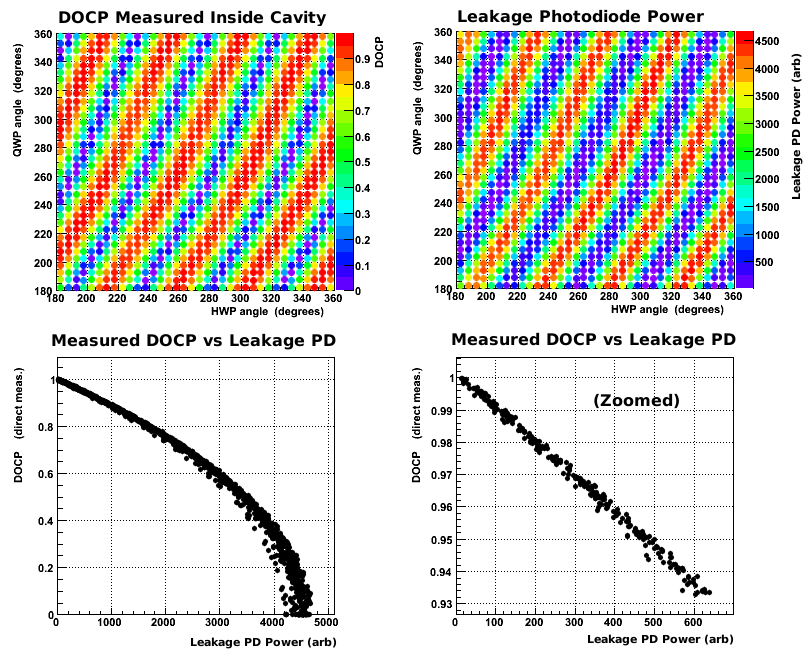
\includegraphics[width=5.6in]{./Pictures/Measured_DOCP_correlation.png}
\caption{\label{fig:DOCP_measured_correl}(Top Left) Degree of circular polarization measured inside the optical cavity as a function of wave plate rotation angles. (Top Right)Leakage photodiode power measured over same scan of wave plates. (Bottom Left)Measured correlation of DOCP inside optical cavity and leakage photodiode power. (Bottom Right)Measured correlation of DOCP inside optical cavity and leakage photodiode power zoomed in to the region near 100\% DOCP.}

\end{figure}
\begin{figure}[ht]
\begin{center}
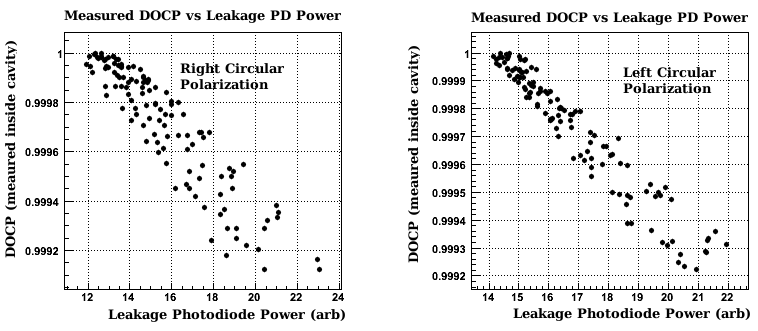
\includegraphics[width=5.9in]{./Pictures/zoomed_correl.png}
\caption{\label{fig:landr_docp_correl}Correlation of left and right circular polarization states directly measured inside the unlocked optical cavity versus power in the leakage photodiode. Statistical uncertainty near 100\% DOCP is shown in the worst case (right circular polarization) to be 0.02\% full width.}
\end{center}
\end{figure}
 
In conclusion, the issue of inaccurate exit and entrance line transfer matrices can thus be bypassed by analyzing the reflected beam. The laser polarization state was set up using a combination of a linear polarizer (polarizing beam splitter), a QWP and a HWP (see Figure \ref{fig:optical_schematic}). This combination allows any arbitrary state of elliptical polarization to be created. The optimal rotation of the two wave plates is found by minimizing the power in the leakage photodiode. One can think of this process as adjusting the waveplates to effectively cancel the effects of residual birefringence in the remaining optics producing 100\% circularly polarized light at the entrance to the cavity.

The justification of this method is rooted in reversibility theorems for polarization states of light and can be found in \cite{Vansteenkiste} as well as the original papers by R. C. Jones \cite{Jones1}\cite{Jones2}. The most relevant theorem proved in this paper\cite{Vansteenkiste} states that linearly polarized light entering an unknown optical system will emerge as circularly polarized if and only if the same beam retroreflected directly back along the same path in the reverse direction through the optical system emerges in a linearly polarized state orthogonal to the original input linear polarization. The unknown optical system is once again restricted to polarization rotators and birefringent elements represented by unitary matrices, although the arguments hold for elements with polarization independent losses. Imagine an optical setup similar to the one in Figure \ref{fig:reversibility} with incoming polarized light beam ${\bf E_1}$ going through an unknown optical system before emerging as ${\bf E_2}$. Polarization state ${\bf E_2}$ is reflected directly backward as ${\bf E_3}$, traverses the unknown optics in the reverse direction and emerges as vector ${\bf E_4}$. This theorem states that for ${\bf E_1}$ linearly polarized, ${\bf E_2}$ will be circularly polarized if and only if ${\bf E_4}$ is linearly polarized in the direction orthogonal to ${\bf E_1}$. In terms of the optical setup for the Compton photon target, the linear polarizer produces a (horizontal) linearly polarized beam which then goes through a series of optical components before reaching the optical cavity. The fraction of the beam that is circularly polarized at the entrance to the optical cavity will be retroreflected back reaching the linear polarizer as vertically polarized light and be deflected into the reflected photodiode. Linearly polarized light at the cavity will arrive at the linear polarizer as horizontal linear polarization and be measured in the leakage photodiode . Thus, minimizing the leakage photodiode signal will maximize circular polarization at the optical cavity.

\begin{figure}[ht]
\centering
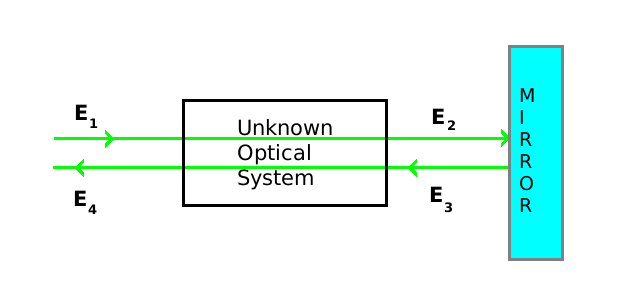
\includegraphics[width=4in]{./Pictures/reversibility_nc.png}
\caption{\label{fig:reversibility}Simple optical setup to illustrate the polarization optical reversibility theorems as seen in \cite{Vansteenkiste}. Polarized light ${\bf E_1}$ goes through an unknown optical system is reflected by a mirror and goes back through the same optical system in reverse emerging as ${\bf E_4}$.}
\end{figure}
\subsection{Determination of Polarization and Error}
Having demonstrated the possibility of achieving 100.00\% circular polarization it is now essential to determine what actually was achieved during Run 2 of the \Qs experiment. Since the leakage photodiode is most sensitive to the circular polarization of the laser in the optical cavity this analysis will focus solely on the signals seen by this photodiode. The discussion will first outline the method for determining the laser polarization. This will be followed by a discussion of possible systematic errors introduced by assumptions or requirements of the method.

\subsubsection{Methodology}
The lower left plot of \ref{fig:DOCP_measured_correl} shows that maximum DOCP does not coincide with zero in the leakage photodiode, indicating that the polarization signal is being added to a background that may or may not be constant. To find the true polarization signal, that is, the portion of the signal in the photodiode correlated with polarization, one must find a way to determine this background. The most obvious source of this background is back-reflections from optical elements downstream of the leakage photodiode. Given the configuration shown in Figure \ref{fig:tablelayout} one can see the linear polarizer, a lens, the waveplates and the vacuum window could easily provide such a background. It is important to take note of the position of the ``flipper mirror'' labeled as 8 in the figure. This mirror was used to deflect the laser into a beam dump periodically to measure backgrounds in the photon and electron detectors. The same flipper mirror is shown also at 8* in diagram (\ref{fig:tablelayout}) reflecting the final configuration of the optics at the end of Run 2 where the flipper mirror was moved just upstream of the periscope. At this position the back-reflections from optical elements installed between it and the leakage photodiode which are all potential sources of back-reflection background in the leakage photodiode remain even when the flipper mirror is inserted to block the beam. Thus the flipper-mirror-inserted signal in the leakage photodiode is a good measure of the background. For the period before the flipper mirror position was optimized for background subtraction, the background must be estimated by other means.

Consider a theoretically optimized optical cavity with a perfectly mode-matched laser. When this cavity is stably locked nearly 100\% of the light is coupled in, leaving no reflected light. Thus, the locked cavity signal in the leakage photodiode becomes a good measure of the background, and the difference between unlocked and locked is the polarization signal. For the optical cavity used in the Compton polarimeter, the coupling was typically 60-80\%. A sophisticated analysis could be attempted to multiply the difference between unlocked and locked by the reciprocal of the coupling to obtain a more precise polarization signal. Instead, what is done in this analysis is to simply assume a conservative 50\% coupling and estimate the polarization signal as 2$\times$ the difference between locked and unlocked as follows:
\begin{equation}
Polarization~Signal = \frac{\left[PD_{leakage}(unlocked)-PD_{leakage}(locked)\right]}{0.5}.
\label{eq:pol_sig}
\end{equation}

The reason this estimate is valid is that the polarization signal is used, not to measure the laser polarization, but to set an upper bound on how far it could have strayed from the assumed 100.00\% circular polarization. Even with conservative estimates of the error, the polarization will be shown to be constrained at the $< 0.2\%$ level.

Figure \ref{fig:rrpd_vs_time} shows the signal of the leakage photodiode over Run 2\footnote{Note that the leakage photodiode sits behind a turning mirror and is positioned to catch only backward traveling light. It is calibrated to milliwatts of light incident on the mirror.  The actual power entering the integrating sphere is down from this by about 2 orders of magnitude, thus this measurement is potentially sensitive to ambient light sources. The integrating sphere is close to the mirror but not completely shielded to prevent light from sources other than the reflected beam from entering. Light that enters from other sources such as glow in the mirror produced by the forward going beam are not subject to the same attenuation and will likely be overestimated by a factor of something like 100$\times$. These are all part of the background that must be subtracted.}. As explained in the caption, the signal has three levels, the lowest when the flipper mirror is inserted, the intermediate level when the flipper is retracted and the optical cavity locked and the highest level when the optical cavity is unlocked. The difference between the two upper bands in the diagram (unlocked-locked) is the polarization signal estimate as given in Equation \ref{eq:pol_sig}. The dataset has been subdivided into periods where a similar polarization signal is observed. These periods are labeled ``a'' to ``e'' in the Figure \ref{fig:rrpd_vs_time}. For periods ``a'' through  ``c'' the flipper mirror is positioned directly downstream of the leakage photodiode and the polarization signal must come from the estimated value in Equation \ref{eq:pol_sig}. After the flipper is moved downstream in period ``d'', the back-reflections from optical elements downstream of the leakage photodiode are still present when the flipper is inserted allowing the polarization signal to be obtained from the straight difference between flipper in and cavity unlocked, that is, the difference between the bottom and top bands\footnote{Back-reflections from the vacuum window will still be blocked. It is likely then that the polarization signal found by subtracting the flipper-in signal from the unlocked and flipper-out signal will be over-estimated. Thus, the error can only be overestimated.}. This is cleaner and avoids the overestimate of multiplying the unlocked-locked by a factor of 2. Table \ref{tab:pol_sig} gives the polarization signal estimates for the 5 periods of interest.

\begin{table}[!!h]
\begin{center}
\caption{\label{tab:pol_sig}Polarization signal estimates for periods labeled ``a'' to ``e'' in Figure \ref{fig:rrpd_vs_time}. Implied polarization shifts are calculated using Equation \ref{eq:leakage_to_DOCP} with maximum leakage signal of 6300~mW as explained in the text. Method column shows how the polarization signal was calculated for a given period. Period ``d'' was the only time when the difference between unlocked and blocked (shutter inserted) was a valid measure of the polarization signal.}
\begin{tabular}{l|c|c|c|c}\hline
Period&Hour Range&Polarization Signal&Method&Implied $\Delta$DOCP\\ \hline
a&0 - 1065&4-6 mW&Eq. \ref{eq:pol_sig}&0.03\% -- 0.05\%\\
b&1065 - 2100&6-8 mW&Eq. \ref{eq:pol_sig}&0.05\% -- 0.06\%\\
c&2100 - 2575&8-10 mW&Eq. \ref{eq:pol_sig}&0.06\% -- 0.08\%\\
d&2575 - 2943&10-14 mW&$Unlocked-Blocked$&0.08\% -- 0.10\%\\
e&2943 - 3100&4-6 mW&Eq. \ref{eq:pol_sig}&0.03\% -- 0.05\%\\\hline
\end{tabular}
\end{center}
\end{table}  

The zoomed (lower right) plot of measured degree of circular polarization (DOCP) versus leakage photodiode power in Figure \ref {fig:DOCP_measured_correl} provides a linear correlation which can be used to translate measured polarization signal into actual shifts in circular polarization. The slope of the linear relationship is $-0.5\%$ change in DOCP per 45 channels increase in leakage photodiode. The lower left plot in Figure \ref {fig:DOCP_measured_correl} gives the normalization of 4500 channels at maximum leakage photodiode power. This maximum happens when the laser is 100\% linearly polarized at the entrance to the optical cavity. Every 1\% shift in leakage photodiode power relative to the maximum gives a 0.5\% shift in DOCP yielding the following empirical relationship:
\begin{equation}
Cavity~DOCP = 1-0.5\times\frac{Polarization~Signal}{Maximum~Leakage~PD~Signal}.
\label{eq:leakage_to_DOCP}
\end{equation}

\begin{landscape}
\begin{figure}
\centering
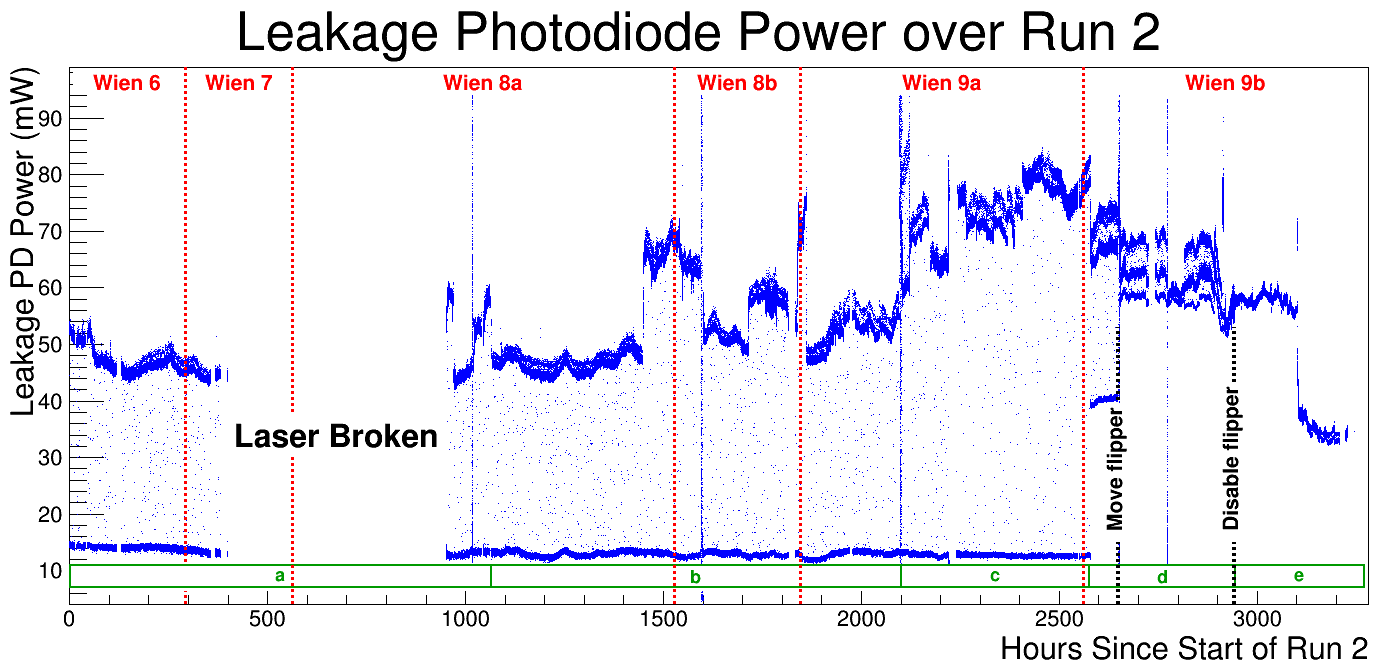
\includegraphics[width=9in]{./Pictures/LeakagePDvsTime_Run2.png}
\caption{\label{fig:rrpd_vs_time}Leakage photodiode versus hours from beginning of Run 2 of \Qs experiment. The triple valued signal comes from flipper mirror inserted (lowest signal), flipper out and cavity locked (intermediate signal) and flipper out and cavity unlocked (largest signal). Twice the difference between the top two values is used as an upper bound for the polarization signal (see Equation \ref{eq:pol_sig}).  Red vertical lines show Wien state divisions used in analysis of the \Qs dataset. Notice the background change after flipper mirror moved. This allowed back-reflections from downstream optical elements to remain when the flipper was inserted providing a measure of the background seen by the photodiode. Near the end of the run the flipper was disabled to mitigate heat load changes on optical elements that were affecting cavity lock stability and mode-matching. Periods of similar estimated polarization signal are labeled a to e.}
\end{figure}
\end{landscape}

There is no direct measurement of the maximum value of the leakage photodiode. Sending the full power of the beam back to the laser head damages the laser and makes it unstable. This practice was avoided, although a couple of mistakes were made, where, for short periods, this happened. One such time when it happened, the leakage photodiode reached the upper limit of the ADC voltage range with a reading of 5.4~W. With $\sim$10.5~W coming from the laser, it seems safe to assume that more than 7~W makes it back to the mirror in front of the leakage photodiode when the waveplates are set to maximize leakage photodiode signal. Allowing a 10\% error in the calibration of the photodiode gives a conservative effective maximum of 6.3~W. Even with this conservative estimate, for the largest polarization signal of 14~mW in period ``d'', this implies a shift in DOCP of only 0.11\%. The total polarization shifts implied by the polarization signals are given in Table \ref{tab:pol_sig}.

To summarize, in the setup used for the Compton polarimeter, the leakage photodiode is sensitive to the degree of circular polarization at the entrance to the optical cavity.  When the laser polarization at the entrance to the optical cavity is close to 100\% circular, the polarization signal (the part of the signal in the leakage photodiode that is sensitive to polarization) is proportional to the DOCP. Direct measurements determined the relationship between polarization signal and changes in DOCP at the cavity entrance to be 0.5\% change in DOCP for every 1\% change in the leakage photodiode power (relative to what its reading would be at maximum returning laser power). This relationship, along with methods outlined for conservative estimates of the polarization signal, is used to bound shifts in DOCP to $<0.11$\%. Thus the polarization is reported to be 100.00\% with possible fluctuations as large as 0.11\%. Several potential sources of systematic error introduced by assumptions of this method are discussed next. 

\subsubsection{Potential Systematic Errors}

The method outlined in the previous section overlooks a few small potential sources of systematic error. These errors naturally fall into two general categories. The first category of systematic error arises from the assumption of a 100\% polarized laser beam incident on the cavity. This assumption is implicit in the use of the Jones calculus, which is only applicable to fully polarized light. An upper bound on the amount of unpolarized light entering the optical cavity will be provided in this section. The second category of systematic errors arises from differences between the optical cavity locked and unlocked states. Although the method outlined in the previous paragraphs is guaranteed to maximize circular polarization at the entrance to the optical cavity, an uncertainty will be assigned to account for any changes in the polarization of the light in the locked cavity after 200+ mirror bounces. The polarization could change by either birefringence of the cavity mirrors creating linear polarization or by incoherent scattering producing an unpolarized component. Furthermore, ambient light levels on the table may contribute marginally to the reading in the leakage photodiode. In particular, shifts of the ambient light between locked and unlocked cavity states and between flipper in and out states may change the ambient light seen by the leakage photodiode, and either accentuate or cancel the true polarization signal, depending upon the sign of the shift.\\
{\bf 1. Unpolarized Light}\\
An unpolarized beam of light has randomly oriented electromagnetic fields as opposed to a polarized beam with well-defined orientations. Since the laser in this system passes through a linear polarizer, it begins in a well-defined and fully polarized state. Depolarization of a fully polarized beam can happen when the beam encounters random scattering centers such as imperfections/residue on the surface of mirrors. The issue of unpolarized light is two-fold. First, is the issue of unpolarized laser light incident on the optical cavity (depolarization occurring before the optical cavity) and second is the issue of depolarization that occurs inside the optical cavity. 

The issue of unpolarized light incident on the optical cavity was addressed by direct measurement inside the optical cavity region (with the cavity unlocked). An upper bound of 0.04\% unpolarized light was determined. This means that light that arrives at the optical cavity is at least 99.96\% polarized. This measurement did not bound the depolarization inside the locked cavity. Depolarization that happens before the optical cavity will be measured equally on both the locked and unlocked signals in the leakage photodiode and will thus be absent from their difference whenever the polarization signal is computed using Equation \ref{eq:pol_sig}. 

Depolarization that happens inside the cavity will only show up on the locked signal and will inflate the locked signal in the leakage photodiode falsely diminishing the polarization signal computed using Equation \ref{eq:pol_sig}. This issue of depolarization inside the locked cavity will be discussed in the next section on errors arising from differences between locked and unlocked states. It will be shown that data taken during period ``d''  can be used to bound the effects of both incident unpolarized light and intracavity depolarization. Although this data provides an even tighter bound on incident unpolarized light, the more conservative (and directly measured) 0.04\% bound was included in the error in Table \ref{tab:pol_error} to account for depolarization.

{\bf 2. Differences between Locked and Unlocked Cavity}\\
The remaining sources of error concern unknown differences between locked and unlocked optical cavity states on the laser table. Three sources of potential differences between the two states will be considered and arguments made to bound each. The three sources are as follows: increases in linear polarization that occur inside the locked optical cavity due to residual birefringence of the reflective coating on the cavity mirrors; ambient light shifts (or changes in background) between locked and unlocked states; and depolarization that occurs inside the optical cavity. 

The degree to which shifts in ambient light affect the polarization signal would be best found by direct measurement on the laser table by isolating the leakage photodiode from all ambient light except that which comes through the mirror. If the ambient light seen by the leakage photodiode increased when the cavity locked, this effect would inflate the locked signal and partially cancel the polarization signal which was measured as unlocked minus locked. The author believes this is a negligible effect but it would be best to directly measure or eliminate it in the future. Furthermore, if the polarization state changes when the cavity locks, either by depolarization inside the cavity or an increase in linear polarization from birefringence on the cavity mirrors, this too would, at least partially, cancel the polarization signal by adding signal in the leakage photodiode only in the locked state. It is a difficult task to disentangle these three effects (linear polarization inside the cavity, depolarization inside the cavity and ambient shifts) without direct measurement. A measurement was made to bound the change in polarization of the laser between the locked and unlocked cavity states. Evidence is provided in the following paragraphs that this measurement along with data taken during \Qs is sufficient to bound errors from each of these effects on the circular polarization inside the locked cavity.

Evidence for polarization changes with cavity lock may be present in deviations from the expected signal level seen in the leakage photodiode. The polarization signal estimated as the difference between unlocked and locked divided by coupling (Equation \ref{eq:pol_sig}) assumes that the only change visible to the leakage photodiode when the cavity locks is a change in reflected {\bf power}. Under this assumption, the polarization signal, that is, the signal after the polarization-independent background has been subtracted, is simply the difference between unlocked and locked scaled by 1/coupling to estimate what would be measured with 100\% of the power coupled into the cavity. However, the leakage photodiode is sensitive to both polarization and power changes. On the other hand, the reflection photodiode is sensitive to power but insensitive to small changes in polarization and ambient background light. Thus, the fractional drop in power in the reflected photodiode is used as a measure of the coupling into the cavity. Comparing the changes in both of these photodiodes allows one to test the assumption of a ``power-only'' change in the leakage photodiode between locked and unlocked. If the laser polarization does not change when the cavity locks\footnote{This means that the intracavity polarization is the same as it was measured to be at the entrance to the cavity and multiple bounce reflections from cavity mirrors do not change polarization.}, then one might expect an identical fractional shift in both the leakage and reflection photodiodes. An identical fractional shift would provide evidence (although not conclusive) that the shift is solely due to the power of the reflected beam. Figure \ref{fig:rpd_rrpd_overlay} shows an example of the leakage photodiode signal over a half hour period during Run 2. A scaled reflection photodiode signal has been overlayed to demonstrate the expected locked signal level due to power shifts in the reflected beam. The small excess of $\sim0.5$~mW in the locked leakage photodiode above what is expected from the change in reflected power may be attributed to a change in either polarization or ambient background light or to a combination of both. With this hint of a polarization/ambient light shift with cavity lock, it becomes necessary to bound these effects.
 
\begin{figure}
\centering
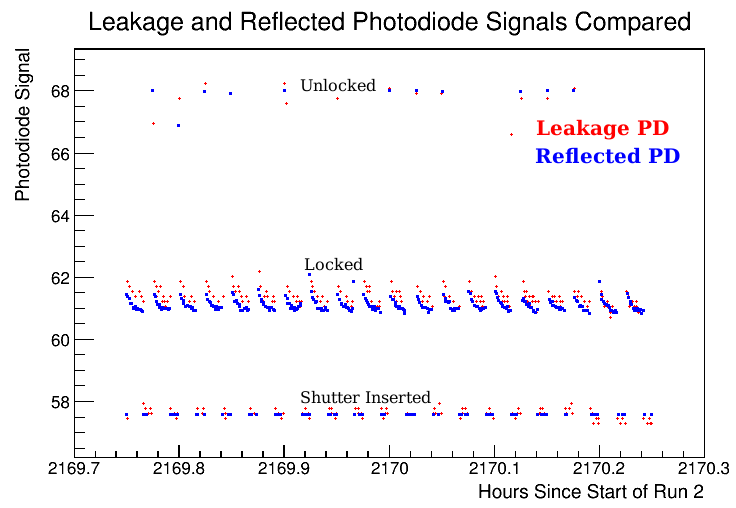
\includegraphics[width=5in]{./Pictures/RPD_RRPD_overlay.png}
\caption{\label{fig:rpd_rrpd_overlay}Zoomed in section of Figure \ref{fig:rrpd_vs_time} showing the leakage photodiode signal levels in milliwatts for unlocked, locked and shutter inserted. Overlayed is a scaled and offset reflection photodiode signal to demonstrate the expected signal change from power only. A small 0.5~mW excess signal can be seen in the leakage photodiode. }
\end{figure}

A dedicated measurement was made after Run 2 of \Qs was completed to bound the difference between locked and unlocked polarization. In this test, the laser transmitted through the cavity in both locked and unlocked states was polarization analyzed. This measurement was possible when the cavity was unlocked due to the relatively low reflectivity of the mirrors ($R=99.5\%$). The results, shown as a function of laser power in Figure \ref{fig:pol_change}, are consistent with no difference in circular polarization between locked and unlocked cavity states as measured on the transmitted beam in the exit line. For these measurements the linear polarization of the transmitted beam was measured in the exit line by rotating a linear polarizer and measuring the power transmitted through the polarizer as a function of rotation angle. A sinusoidal fit to the data of transmitted intensity versus rotation angle was then used to calculate the degree of linear polarization as DOLP = amplitude/constant offset. Circular polarization is then calculated as
\begin{equation}
DOCP =\sqrt{1-DOLP^2}
\label{eq:DOCP}
\end{equation}
 under the assumption of 100\% polarization, that is, that no light is unpolarized. Even if one were to argue that a small difference in DOCP is observed, it is important to keep in mind that the measurements in this figure are taken in the exit line where the DOCP is around 97.6\%, the value that roughly translates into 100\% polarization in the optical cavity \footnote{The polarization state of the light is changed by the turning mirrors and vacuum window encountered between the optical cavity and the exit line. Thus, 100\% circularly polarized light in the optical cavity is measured as approximately 97.6\% circularly polarized in the exit line.}. Suppose one were to conservatively estimate a circular polarization change as high as 0.2\% between locked and unlocked states in the exit line from Figure \ref{fig:pol_change}. The sensitivity of DOCP to changes in linear polarization is given by
\begin{equation}
\frac{d DOCP}{d DOLP} =\frac{-DOLP}{\sqrt{1-DOLP^2}}.
\label{eq:DOCP_sens}
\end{equation}
Thus the sensitivity in the exit line to shifts in linear polarization is 
\[\frac{dDOCP}{dDOLP}\rvert_{(DOCP=97.6\%)}=-0.223,\] whereas the sensitivity in the cavity is closer to \[\frac{d DOCP}{d DOLP}\rvert_{(DOCP=99.9\%)}=-0.0474\] giving almost a factor of 5 suppression\footnote{This assumes an identical shift in linear polarization both in the exit line and inside the cavity. A more sophisticated model would utilize a measured optical transfer matrix to translate the change measured in the exit line to that inside the cavity. However, this estimate of suppression is valid to first order under the assumption that the exit line optics create small changes in laser polarization.}. Even a shift as large as 0.2\% in DOCP in the exit line would translate to only a 0.04\% shift of DOCP inside the cavity.

The previous method utilizes a rotating linear polarizer to measure laser linear polarization which then implies a circular polarization under the assumption of no depolarization (Equation \ref{eq:DOCP}). One could argue that the above measurement provides a bound on shifts in linear polarization not circular polarization since linear polarization is what is actually measured. Circularly polarized light and unpolarized light will be indistinguishable when analyzed by a rotating linear polarizer. The conservative 0.2\% shift in DOCP measured in the exit line implies a 0.9\% change in linear polarization in the exit line. It is safe to assume to first order that this also implies a shift of approximately 0.9\% inside the cavity as well, setting an upper limit of $\Delta$DOLP$<0.9\%$ between locked and unlocked. Table \ref{tab:pol_error} includes a 0.04\% error associated with the implied shift in intracavity DOCP from a 0.9\% increase in linear polarization.

\begin{figure}[ht]
\begin{center}
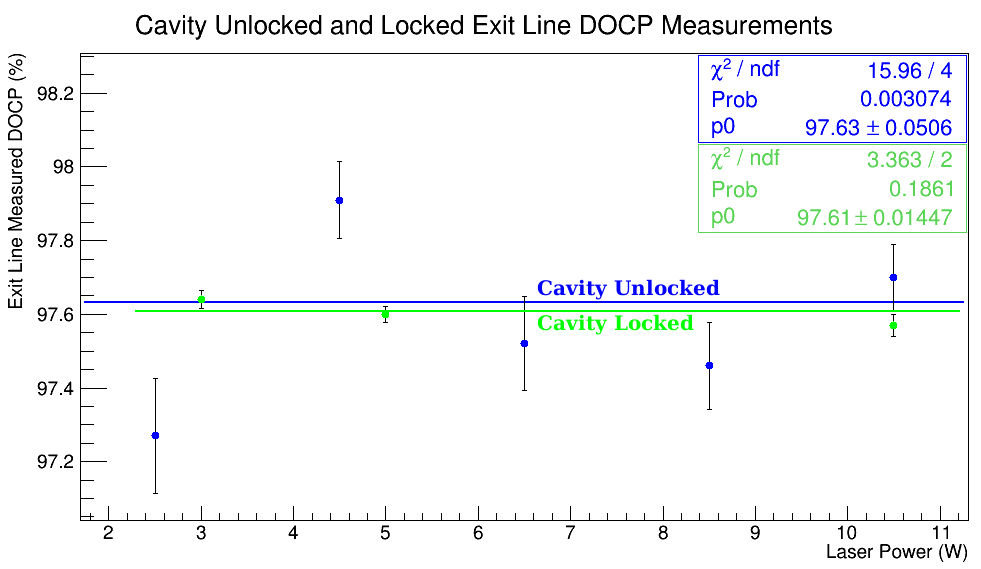
\includegraphics[width=5.0in]{./Pictures/UnlockedPolChange.png}
\caption{\label{fig:pol_change}Laser polarization measured in the exit line for both cavity locked and cavity unlocked. Cavity mirrors with reflection coefficients R=99.5\% allow enough light through even in the unlocked state to measure polarization although the accuracy is reduced. The difference in polarization between locked and unlocked is statistically consistent with zero.}
\end{center}
\end{figure}

The two remaining potential sources of error, depolarization inside the locked cavity and ambient light shifts on the laser table between locked and unlocked states, can be bounded indirectly by a combination of plausibility arguments and data. Direct measurement inside the optical cavity confirmed that 100.00\% DOCP was achievable for both left and right circular polarization states at a statistical uncertainty level of $\pm 0.02\%$ (see Figure \ref{fig:landr_docp_correl})\footnote{The upper limit of $\pm 0.04\%$  for unpolarized light actually limits the accuracy of the measured correlation in Figure \ref{fig:landr_docp_correl}. The slope remains the same but the maximum shifts down when there is an unpolarized component. The method used to measure circular polarization in the correlation plot also assumes 100\% polarized light and cannot differentiate between circularly polarized and unpolarized light. }. When the system is optimized, that is, the minimum signal in the leakage photodiode is achieved by adjusting the rotation angles of the waveplates, this minimum signal corresponds to 100.00\% DOCP (see Figure \ref{fig:landr_docp_correl}). One such waveplate optimization scan was executed during period ``d''. The results of this optimization can be seen in Figure \ref{fig:LCPandRCP}. As illustrated in the figure, the polarization signal was greatly reduced by the scan. The total difference in leakage photodiode signal between unlocked and blocked (flipper inserted) can be used to place a tighter bound on depolarization at the entrance to the cavity than even the direct measurement of $<0.04\%$. Using Equation \ref{eq:leakage_to_DOCP} with a 2~mW polarization signal from the unlocked minus blocked in Figure \ref{fig:LCPandRCP} gives an upper bound on this source of depolarization of 0.02\%. Neither ambient light nor depolarization are waveplate dependent, thus the fact that the optimization reduced both locked and unlocked leakage signals shows that both had a valid polarization signal that could not be mocked by ambient light or depolarization. At the end of the optimization, the locked signal was about 1~mW less than the unlocked and the blocked (flipper inserted) signal was about 1~mW below the blocked. If depolarization inside the cavity were a large effect, one might expect the order to be inverted and the unlocked signal to be smaller than the locked after optimization. It is the author's opinion that the ambient light seen by the leakage photodiode is the smallest when the shutter is inserted since the beam is dumped preventing both reflection and transmission of light. In that case, the blocked beam signal is actually an underestimate of the ambient light background and the leakage photodiode signal when the cavity is locked will be composed of any shifts from depolarized light (always a positive addition) and ambient light (also positive by this argument). Thus the measured difference in the leakage photodiode between locked and blocked directly after optimization can be used to bound depolarization giving 
\[
Unpolarized \leq0.5\times\frac{Polarization~Signal}{Maximum~Leakage~PD}=0.5\times\frac{6~mW}{6300~mW}=0.05\%.
\]
The polarization signal was calculated as follows. From Figure \ref{fig:LCPandRCP}, the difference between locked and blocked is about 1.5~mW. Assuming this is totally from unpolarized light, this difference was multiplied by a factor of 2 to allow for the fact that the linear polarizer only transmits half the total unpolarized power. Multiplying by another factor of 2 allows for only 50\% coupling of power into the cavity which implies that 50\% of the reflected beam comes from inside the cavity giving a total of $1.5\times2\times2=6$~mW. This translates into a 0.05\% shift in DOCP. Similarly, if one assumes the total difference between locked and blocked to be from ambient light shifts, the polarization signal is $1.5\times2=3$~mW, which translates into upper bound on error from ambient light shifts of 0.02\%. Table \ref{tab:pol_error} includes a 0.02\% error for possible ambient light shifts and 0.05\% error for depolarization inside the cavity based upon the arguments presented here. 
 
\begin{figure}[!!!!ht]
\begin{center}
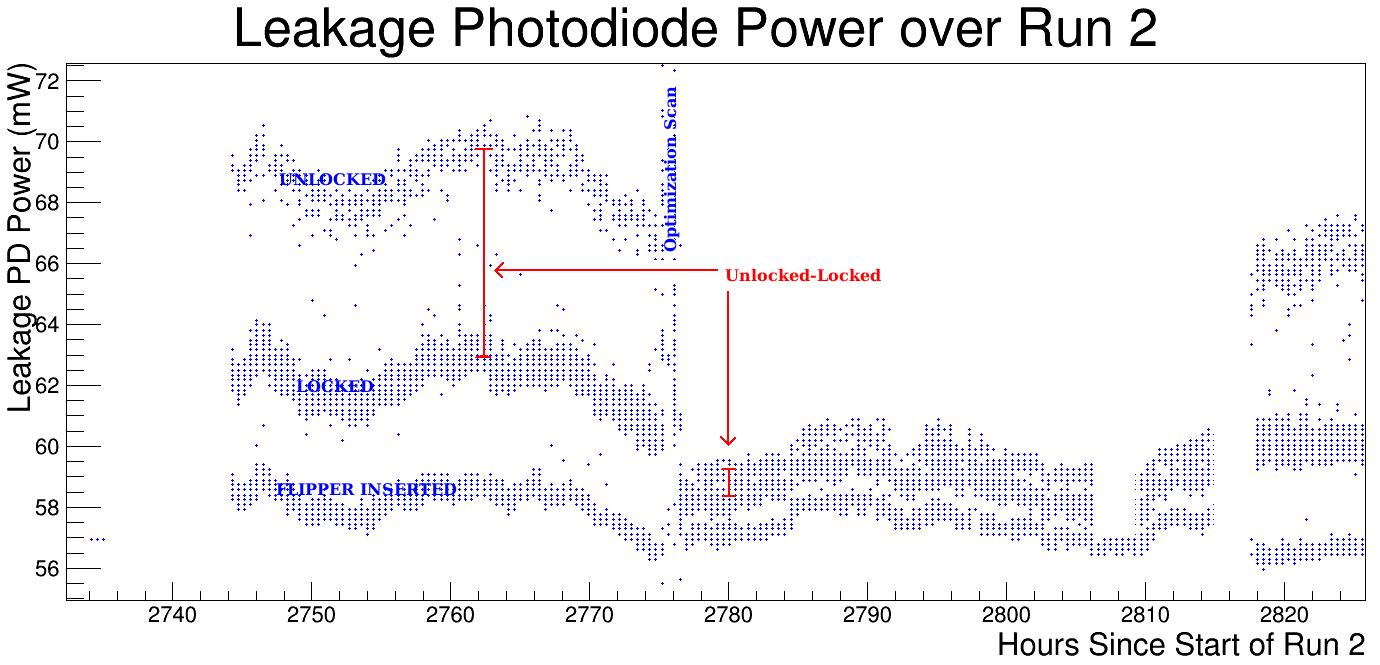
\includegraphics[width=5.5in]{./Pictures/LCPandRCP.png}
\caption{\label{fig:LCPandRCP}Example of optimization scan of half-wave and quarter-wave plates to minimize polarization signal in leakage photodiode. This is a zoomed-in section of Figure \ref{fig:rrpd_vs_time} where the laser helicity state was flipped and an optimization scan was done to find the best position. This was during period ``d''. The polarization signal was about 14~mW before the optimization and less than 2~mW after the optimization.}
\end{center}
\end{figure}


As already alluded to, the reflected beam returning from the locked cavity is composed of both single bounce light from the entrance cavity mirror as well as multiple bounce beam from inside the cavity. A 2011 publication by Peter Asenbaum and Mark Arndt in {\it Optics Letters} describes a setup where the sensitivity of the reflected beam to birefringence of the cavity mirrors is used to create an error signal for maintaining cavity lock \cite{Asenbaum}. It would be useful for future experiments to utilize a modified version of the setup described in this paper to directly measure the effect of cavity mirror birefringence. It is expected to be a tiny effect for \Qs but a direct measurement is more satisfying than a bound.  

To summarize the discussion of systematic error, the polarization signal is used to measure the shifts in DOCP with time. The polarization signal is the part of the reflected laser that is sensitive to changes in polarization of light at the optical cavity. The polarization signal is estimated by taking the difference of unlocked and locked signals in the leakage photodiode and multiplying by 2 to allow for imperfect coupling. The largest polarization signal is seen in period ``d'' where 10-14~mW was recorded. Using the correlation between leakage photodiode signal and DOCP measured directly inside the optical cavity provides a means of translating polarization signals into shifts in DOCP and yields 0.5\% percent change in DOCP per percent change in polarization signal. An error of of 0.02\% associated with the statistical uncertainty of the correlation of DOCP and leakage photodiode signal must also be included \ref{fig:landr_docp_correl}. The largest measured polarization signal of 14~mW implies a laser DOCP change of $\leq 0.11\%$. Since this method assumes that only the power of the reflected beam changes when the cavity locks (as opposed to the polarization of the beam or the ambient background light), upper bounds were established for real changes in intracavity circular polarization due to depolarization ($\leq 0.05\%$) and cavity mirror birefringence ($\leq 0.05\%$) as well as false shifts from ambient backgrounds ($\leq 0.02\%$). Finally, the method used for direct measurement of DOCP in the cavity region versus leakage photodiode power (see Figure \ref{fig:landr_docp_correl}) cannot distinguish between unpolarized and circularly polarized light. If the beam at the entrance to the optical cavity were to have a component that was unpolarized, this would shift the correlation plot downward by the percentage of unpolarized light. The unpolarized component was bounded by direct measurement in the cavity region to be $\leq 0.04\%$. The laser polarization then becomes 100.00\% with a conservatively estimated error of 0.14\%. Table \ref{tab:pol_error} lists the sources and values for each of the error contributions to the laser polarization.

\begin{table}
\begin{center}
\caption{\label{tab:pol_error}Table of errors.}
\begin{tabular}{|l|c|p{7cm}|}\hline
Category&Error&Explanation\\\hline
Polarization Tracking&0.11\%&Error derived from period ``d'' with a maximum polarization signal of 14~mW (see Table \ref{tab:pol_sig}).\\
Model&0.02\%&Statistical variation around linear correlation of DOCP vs. Leakage PD signal (see Figure \ref{fig:DOCP_measured_correl}).\\
Unpolarized Light (unlocked)&0.04\%&Unpolarized light at entrance to cavity. Conservative upper bound from direct measurement. This produces an offset in the correlation plot \ref{fig:DOCP_measured_correl}. Changes in polarization are relative to the maximum which can shift from 100.00\% to as low as 99.96\%.\\
Intracavity $\Delta$DOCP&0.04\%&Implied DOCP shift from change in linear polarization inside locked cavity. Upper bound of 0.9\% shift in DOLP between locked and unlocked. A 0.9\% shift in DOLP would shift DOCP from 99.90\% to 99.86\%\\
Intracavity Depolarization&0.05\%&Depolarization inside locked cavity.\\
Ambient Light Shifts&0.02\%&Difference in ambient light on the laser table between locked and unlocked that mimics polarization signal.\\\hline
{\bf Total}&{\bf 0.14\%}&Quadrature sum of errors.\\\hline

\end{tabular}


\end{center}
\end{table}

\subsubsection{Lessons from Periods of High Polarization Signal}
Before leaving the discussion of laser polarization it is useful to mention three short periods that are outliers with much larger polarization signals. Although, these should be removed from the dataset for calculation of electron beam polarization for \Q, their inclusion will have a negligible effect. 

The first period of non-optimal laser polarization occurred on Feb 25,2012 between 12:00 and 19:00. This period corresponds to hours 2169--2175 on Figure \ref{fig:rrpd_vs_time} but has leakage photodiode signals that are too large to be included in the range of this plot. The polarization signal was as large as 400 channels which implies that the laser polarization was near 97.3\%, polarization--a change easily observed by the electron detector. This period corresponds to a laser polarization scan where the laser polarization was deliberately changed during a period of stable electron beam conditions to verify that the electron detector measurements tracked the predicted laser polarization change from the model. The results of the electron-detector-measured electron beam polarizations while the laser polarization was being scanned can be seen in Figure \ref{fig:las_pol_scan}.
\begin{figure}[ht]
\begin{center}
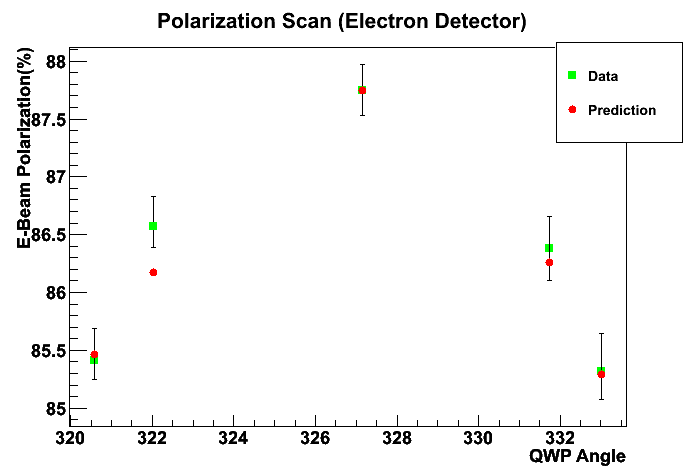
\includegraphics[width=4.0in]{./Pictures/las_pol_scan.png}
\caption{\label{fig:las_pol_scan}Plot of measured electron beam polarizations reported by electron detector while laser circular polarization was scanned by rotating the QWP. The optics model predicted a shift from 100\% to 97.4\% in laser polarization, in good agreement with what was reported by the electron detector. Predicted values normalized to be equal with electron beam value at position of highest laser polarization. The error bars on the electron detector polarizations are only statistical. No model errors are shown for the predicted values.}
\end{center}
\end{figure} 

The second period occurred on Feb 22,2012 15:50 - Feb 23, 2012 11:50 which corresponds to  2100.8 -- 2120.8 hours in Figure \ref{fig:rrpd_vs_time} and  has a difference between locked and unlocked of about 25 mW. This corresponds to a polarization signal of 50 mW and a 0.4\% polarization change. The story of this period according to the electronic logbook is interesting and shows just how sensitive the leakage photodiode is to changing birefringence -- changes that would not be accounted for in the previous method of measuring the exit line transfer matrix. Heating effects had been observed in the optics, which were creating issues with optical cavity mode-matching. When the laser flipper was removed and when the cavity locked, changes in laser power on optical elements were creating shifts in the mode-matching quality of the beam. It was decided to try cleaning optical elements on the laser table. One lens was cleaned and the bottom turning mirror on the periscope replaced. This particular turning mirror was particularly subject to contamination from dust landing on its surface and burning due to its upward facing position. When the laser was once again turned on and locked the polarization signal had increased from $\sim 7$~mW to $45$~mW. Hours later a new scan of half-wave and quarter-wave plates was done to re-optimize the system and the polarization signal once again was reduced to $\sim 7$~mW. This is very interesting because simply cleaning optics and replacing a turning mirror changed the circular polarization inside the optical cavity by 0.3\% near the 100\% DOCP position where sensitivity to changes in linear polarization are smallest. Figure \ref{fig:optics_cleaning} shows the response of the leakage photodiode over this period.

\begin{figure}[ht]
\begin{center}
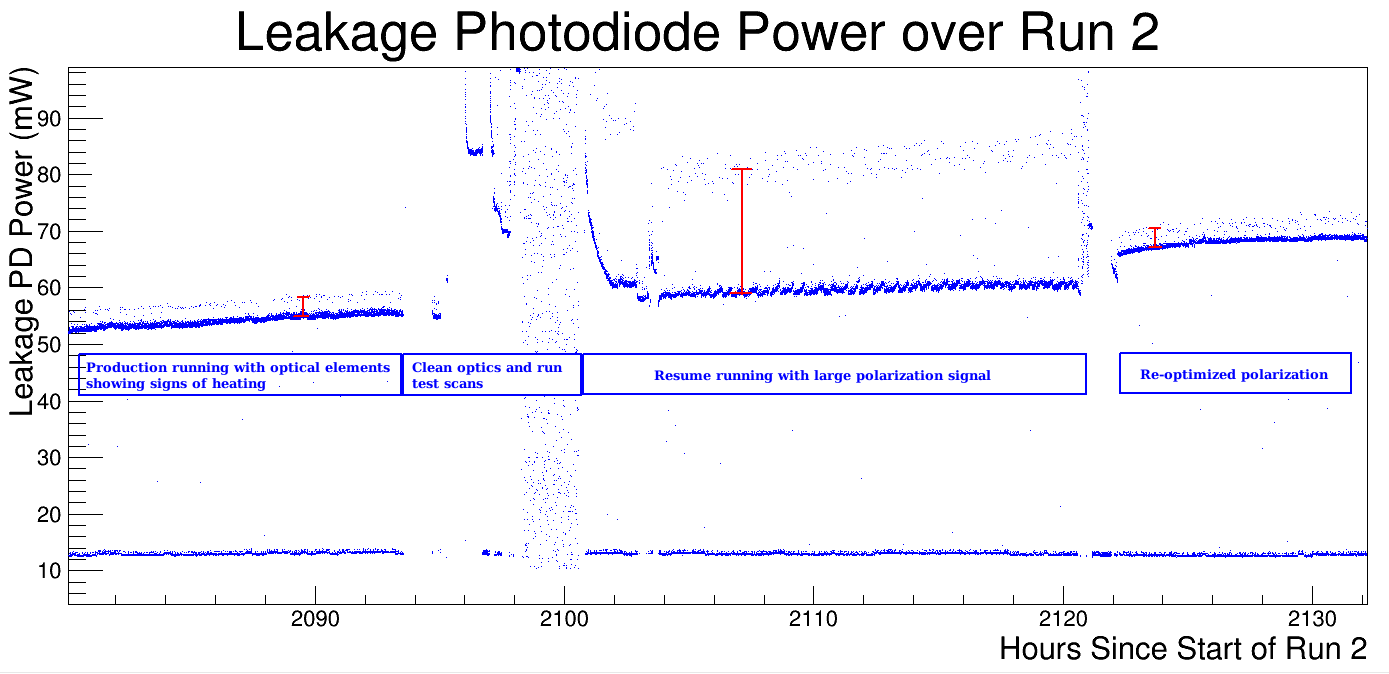
\includegraphics[width=5.5in]{./Pictures/Optics_cleaning_pol_sig.png}
\caption{\label{fig:optics_cleaning}Plot showing leakage photodiode response versus time. A large change in laser polarization is evidenced by the change in polarization signal ($2\times$ red bars) after the optics are cleaned and a turning mirror replaced to mitigate evidence of heating effects. Notice the rapid change in the leakage photodiode for a two hour period after the optical cleaning likely due to residual film on the optics from cleaning.}
\end{center}
\end{figure} 

The final period of large polarization signal is seen on March 27, 2012 between 11:00 and 15:00, which corresponds to hours 2912 to 2916 in Figure \ref{fig:rrpd_vs_time}. This period has a $\sim50$~mW polarization signal. The only evidence of an issue during this time is a laser chiller failure which affects the temperature stabilization of the laser head. Although the temperature inside the laser table enclosure is not recorded, perhaps it increased enough to create small birefringence changes in elements such as the vacuum window. 

In conclusion, the setup on the laser table for the Compton polarimeter worked very well for the creating highly polarized right and left circular states inside the optical cavity. Although laser polarization is a function of time, due to largely unmonitored  processes such as temperature changes, damage to optical components and laser position drift, the leakage photodiode provides a very sensitive measurement of those drifts and provides a bound on polarization drifts at the 0.14\% level. 

Past parity-violation experiments in Hall A at Jefferson lab utilizing Compton polarimetry have relied on exit line polarization measurements and a measured transfer matrix to translate these measurements into intracavity polarizations.  Due to the difficulties inherent in this method as outlined in Section \ref{Sctn:Methodology}, laser polarization has been a significant source systematic error on electron beam polarization measurements for these experiments. The HAPPEX-III experiment quoted a total uncertainty on electron beam polarization of $\pm$0.94\% with the laser polarization uncertainty contributing most of that at $\pm$0.80\% \cite{Friend}. The error budget of \Qs for electron beam polarization was $\pm 1\%$. Although uncertainty in laser polarization of $\pm$0.80\% would have been sufficient for the \Qs experiment, the reduction of this systematic error is a key victory for future parity-violation experiments at Jefferson Lab, such as MOLLER and SOLID, with more stringent requirements for electron beam polarimetry at the $\pm 0.4\%$ level\cite{MOLLER}\cite{SOLID}.

